\documentclass[%
  chapterprefix=false,%
  open=right,%
  twoside=true,%
  paper=a4,%
  logofile={Figures/logo.png},%
  thesistype=master,%
  UKenglish,%
]{se2thesis}
\listfiles
\usepackage[ngerman,main=UKenglish]{babel}
\usepackage{blindtext}
\usepackage[%
  csquotes=true,%
  booktabs=true,%
  siunitx=true,%
  minted=true,%
  selnolig=true,%
  widowcontrol=false,%
  microtype=true,%
  biblatex=true,%
  cleveref=true,%
]{se2packages}

\usepackage{algorithm}
\usepackage{algpseudocode}
\usepackage{multirow}
\usepackage{amsmath}
\usepackage{hyperref}
\usepackage[caption=false]{subfig}
\usepackage{rotating}

\addbibresource{references.bib}
\newcommand\DiffDecMIO{253.71}
\newcommand\DiffGenMIO{31.90}
\newcommand\DiffDecMin{-94.68}
\newcommand\DiffDecMax{-91.76}
\newcommand\DiffGenMin{-96.96}
\newcommand\DiffGenMax{-96.14}

\newcommand\SearchTimeDYNAMOSA{-1.87}
\newcommand\SearchTimeMOSA{-1.22}
\newcommand\SearchTimeWHOLESUITE{-0.95}
\newcommand\SearchTimeMIO{-6.90}

\newcommand\AverageCohen{-0.41}

\newcommand\AverageA{0.40}
\newcommand\MinMod{10}
\newcommand\MaxMod{46}
\newcommand\MinPearson{0.03}
\newcommand\MaxPearson{0.40}
\newcommand\MinSpearmans{0.07}
\newcommand\MaxSpearmans{0.25}




\newcommand{\classname}[1]{\texttt{#1}}
\newcommand{\callable}[2][]{\(\text{\texttt{#2}}(#1)\)}
\newcommand{\field}[1]{\texttt{#1}}

\author{Gonzalo A. Oberreuter Álvarez}
\title{Effects of the Implementation of a Graph-Based Object Synthesis Heuristic \\ on Pynguin}
\degreeprogramme{Computer Science}
\matrnumber{110082}
\supervisor{Prof.\,Dr.~Gordon Fraser}
\external{Prof.\,Dr.~Christian Hammer}
\advisor{}
\department{Faculty of Mathematics and Informatics}
\institute{Chair of Software Engineering}
\location{Passau}

\begin{document}

\frontmatter

\maketitle

\iffalse{}

\authorshipDeclaration{}

\begin{abstract}
  An English abstract to the thesis. 
  TBD.\@
\end{abstract}

\begin{abstract}[german]
  Eine deutschsprachige Zusammenfassung der Arbeit.
  TBD.\@
\end{abstract}

\begin{acknowledgements}
  Some acknowledgements. 
  TBD.\@
\end{acknowledgements}
\fi

\tableofcontents



\mainmatter{}

\chapter{Introduction}\label{chap:introduction}

Software testing is one of the key aspects of software development while trying to ensure quality over a final product, regardless of the context in which the developing process is made.
This quality can be achieved by the insight provided by the result of the tests, and even because of the defects that can be encountered during the testing phase.
Nonetheless, even though coding different kinds of tests is a good practice, it is often ignored by new or inexperienced developers, who also make this mistake halfway by not getting a complete introspection of their own code or, in other words, not getting a complete kind of test coverage.
As of 2017, a study by Trauch and Grabowski~\cite{DBLP:conf/icst/TrautschG17} presented that, over more than 4 million tests, most of them were not correctly categorized (as unit test or not) and approximately half of them use mocking as a testing technique, which tells some aspects about the developing community of the projects in review. 
With this general idea into mind, is that researchers in the last decade   have put effort into autonomous test generation, the concept that implies the usage of different methods or techniques in order to identify patterns and generate test sets with little to zero external intervention.
In 2015, empirical proof was found by Fraser et al.~\cite{DBLP:journals/tosem/FraserSMAP15}, who showed that the usage of automated Java unit test generation increases the general structural coverage, does not lead to the detection of more faults and affects negatively the ability to capture intended class behaviour.
The results of this study state fundamentally that this behaviour  comes from the early stages of the tool in question, and proposes to put more work into the readability of generated tests and  the process of test making itself.

Within the scope of Python testing, Pynguin~\cite{DBLP:conf/icse/LukasczykF22} is command line interface for the generation of unit tests that applies various algorithms for input generation, such as DynaMOSA~\cite{DBLP:journals/tse/PanichellaKT18}, MIO~\cite{DBLP:conf/ssbse/Arcuri17}, MOSA~\cite{DBLP:conf/icst/PanichellaKT15}, Whole Test Suite~\cite{DBLP:journals/tse/FraserA13}, among others.

At the time of its original release (25th of July 2020), Pynguin was a state-of-the-art open source tool that has been the first step for subsequent researches about how to improve the performance and functionalities of Pynguin itself, including CodaMOSA~\cite{DBLP:conf/icse/LemieuxILS23}, PyLC~\cite{DBLP:conf/sac/SalariEAS23} and many other tools that are briefly explained in the Section~\ref{chap:related_work}.
These recent new extensions of Pynguin and the latter aforementioned problem at the time of generating complex object inputs are the principal motivations of this thesis and the related and future work to it.

The original Pynguin research paper~\cite{DBLP:conf/icse/LukasczykF22} stated that after the test generation of 118 Python modules, the average branch coverage over all algorithms was $66.8\%$, which leads to think that improvement is possible.

Although automatic test generation is achievable while having type information available for statically typed languages like Java~\cite{DBLP:journals/tse/FraserA13} or C, dynamically typed languages such as Python, JavaScript or Lua enforce further problems at the time of generating correct arguments for the execution of methods or functions under test.
The major concerns about the argument generation, is that the lack of type information produces ambiguity for the heuristics of the tool at hand at the moment of synthesizing non-primitive types.
Also, the complexity of these class instances in terms of their internal field values might produce runtime errors, which imply a local optima in the search landscape of the test representation~\cite{DBLP:conf/sigsoft/0001O00D21} and therefore an upper bound for coverage.
This latter idea, brings a recurrent problem in the automatic test generation for languages that include any kind of Object-Oriented Programming, which is the reaching of branches that need an object instance as input in a specific variable-state.

\begin{figure}
  \inputminted[linenos]{python}{Figures/example.py}
  \caption{Module example.py\label{lst:1}}
\end{figure}

\begin{figure}
\inputminted[linenos]{python}{Figures/dependencies.py}
\caption{Dependency module of example.py\label{lst:2}}
\end{figure}

\begin{figure}
  \inputminted[linenos]{python}{Figures/test1.py}
  \caption{Test suite generated by Pynguin for module example.py\label{lst:3}}
\end{figure}

As an example, Listings~\ref{lst:1}~and~\ref{lst:2} represent a Module Under Test (MUT) and its dependency module, respectively, in which lines 8, 10 and 12 of the MUT are the targets of the branch coverage problem.
Even though the test suite generated by Pynguin (see Listing~\ref{lst:3}) gets to a branch coverage of \(37.5\%\) (using DynaMOSA, the seed 1998 and 100 seconds as stopping condition), it can be inferred that this result comes from \verb|test_case_1()|, that executes one of the first two branches in the MUT and checks if the variables \verb|actor| and \verb|target| are actual \verb|Player| objects.
This behaviour prevents Pynguin from escaping a local optima for the branch coverage of line 12.

The current Master's thesis proposes an addition to the original structure of Pynguin, specifically to the \classname{GenerationAlgorithm} abstract class, by developing a Graph-Based Object Synthesis approach~\cite{DBLP:conf/sigsoft/0001O00D21} (GBOS from now on) for the static analysis of Python at bytecode level in order to generate suitable object inputs, diminish the branch coverage gap, and empirically study the effect of the presence of type information in this same generation heuristic.

Coming back at Listing~\ref{lst:1}, the idea of using a graph for the synthesis of objects is to get Pynguin to generate a \verb|GameState| object with the necessary \verb|Players| in the \verb|players| list, and an \verb|Action| object with correct attributes, so a hypothetical test could reach the third branch in the MUT, even if it is with a false guard.

The Graph Based heuristic proposed by Lin et al.~\cite{DBLP:conf/sigsoft/0001O00D21} firstly generates an Object Construction Graph (OCG), which is a sub-graph of a previously generated Program Dependency Graph (PDG).
Then, this OCG is used to generate a code template that should be translated directly into the test code representation of Pynguin, for it to be then evolved or modified by one of the available Search-Based algorithms.
Pynguin, similarly to other Search-Based test generating tools, represents its test cases as a sequence of implementations of a super class \classname{Statement} that can be later transformed into an Abstract Syntax Tree (AST) and an actual block of Python code.
At its time, the GBOS heuristic was completely implemented in and for Java, which means that part of the work done was to ideate a Python representations of the OCG.\@
Listing~\ref{lst:4} shows the code of a hypothetical statement sequence template for the testing of the example module, that still gets a run time error in line 18.
However, this template allows Pynguin to get out of the local optima thought mutations, if right values are modified in the correct variables.

\begin{figure}
  \inputminted[linenos]{python}{Figures/template.py}
  \caption{Potential test template obtained through the use of an OCG\label{lst:4}}
\end{figure}

A type information gathering mechanism (e.g.~the analysis of every method or function's AST) is applied throughout the study in order to review the modules in the testing set of the experimental setup on how the general type information of a Python module correlates with the ability of the GBOS approach to generate correct object inputs templates and its results.
The reason for this is, as stated before, Python being a dynamically typed language and not requiring the type of variables in the script in order to be executed.
To illustrate this, if line 4 in Listing~\ref{lst:1} were to be replaced to \mint{python}|def checkRules(self, action, state) -> bool:| it would make Pynguin not have any information about the type of the parameters, and generate a test suite similar to the one in Listing\ref{lst:5}.
The behaviour that allows Pynguin to generate the previous suite imply that the current type system implemented as part of it does not work completely well when trying to infer object types.
Therefore, this idea tries to measure the coverage result effect of the variable amount of type information available.

\begin{figure}
  \inputminted[linenos]{python}{Figures/test2.py}
  \caption{Test suite generated by Pynguin for a variation of module example.py\label{lst:5}}
\end{figure}

After the implementation part was done, a study of the extension was made through the selection of arbitrary sets of Python modules, being these a combination of the ones used for various studies done to Pynguin's updates over time.

As a summary, the main contributions of this study are

\begin{itemize}
  \item An implementation of the GBOS heuristic described by Lin et al.~\cite{DBLP:conf/sigsoft/0001O00D21} as an extension to the automatic test generation tool for Python, Pynguin.
  \item An empirical analysis over the effects of the usage of the GBOS heuristic, when run on a set of Python modules that aim to generalize the current state of publicly available modules.
  \item The discussion about the different implications that come when using the GBOS extension, and the possible future improvements to it.
\end{itemize}

The Pynguin extension can be found, together with the example module presented in the current section, in the same GitLab repository of Pynguin, under the branch named ``GBOS''.

\chapter{Background}\label{chap:background}

\section{Automatic Test Generation}

Software testing is widely recognized among developers as a good practice, when developing any kind of software.
This comes from the benefits, in terms of bug finding and correct functionality, that writing good software tests brings.
Anyhow, the latter adjective ``good'' is subjective as a concrete measure, and often replaced for a fitness metric, such as coverage.

Code coverage can be represented in many ways, such as the amount of lines that are executed when running a test suite, the amount of branch-decisions that are taken or the amount of lines that are checked when evaluating the validity of a test assertion.
Although these fitness functions are clearly defined, it is usually difficult and time-consuming for developers to come up with enough or high quality test cases that cover in terms of coverage their respective software completely.
This drawback appears when a software is updated with dead code, or is not written at the same time as its test cases, which are strong enough reasons to think of automatic test generation as a viable general-case alternative.

Since at least the past two decades, there has been a collective effort to shrink the necessity for handwritten software tests, with the development of tools and techniques related to evolutionary algorithms~\cite{DBLP:conf/sigsoft/FraserA11}, software static analysis~\cite{DBLP:conf/osdi/CadarDE08}, and (in a more current solution) large language models~\cite{DBLP:journals/corr/abs-2207-10397}.
Usually, automatic test generation is portrayed as an optimization problem, that takes test cases or test suites as solutions to the task of maximizing the fitness coverage of a module under test and minimizing the amount of test cases/statements within a test suite.
In this scenario, the greatest obstacles are finding a correct representation of a test case for the chosen programming language, and finding a suitable way of going through the domain's search space.

\newpage

\section{Program Slicing}\label{sec:slicing}

While being part of the studied heuristic, program slicing is the technique of obtaining a subset of program statements according to a point of interest inside the program at hand.
Within the scope of the GBOS heuristic, the type of slicing that bring the most interest is static slicing, which is done merely with the information that can be obtained statically from a program.
Although slicing is a quite versatile tool, it is mostly used and related to the Program Dependence Graph (PDG), structure that represents all dependencies between statements or blocks in a program.

A Control Flow Graph (CFG), is the first step to the gathering of data flow inside a program, as it defines the explicit jumps between statements.
It can be defined as \(\text{CFG} = \langle V_{\text{CFG}}, E_{\text{CFG}} \rangle\) where every node represents an abstraction of statements or basic blocks and every directed edge, a path of execution.

The Control Dependence Graph (CDG) is the second relevant structure working as a requisite for slicing.
Before defining the elements of a CDG, it is necessary to define the concepts
\begin{itemize}
  \item \textbf{Dominator}: a statement \(v_1\) dominates another statement \(v_2\), if every execution path to \(v_2\) in the CFG goes through \(v_1\).
  \item \textbf{Post-Dominator}: a statement \(v_1\) post-dominates another statement \(v_2\), if every execution path from \(v_2\) to an exit node in the CFG goes through \(v_1\).
\end{itemize}
Then, a \(\text{CDG} = \langle V_{\text{CDG}}, E_{\text{CDG}} \rangle\) is a graph where \(V_{\text{CDG}} = V_{\text{CFG}}\), and for every pair \(v_1, v_2 \in V_{\text{CDG}}\), there is a directed edge \((v_1, v_2)\) if and only if \(v_2\) is not a post-dominator of \(v_1\) and there is a path in the \(CFG\) between \(v_1\) and \(v_2\) whose nodes are not post-dominated by \(v_2\).
This edge represents a control dependency between both statement blocks.

Similarly, the data dependencies of a program can be represented with a Data Dependence Graph \(\text{DDG} = \langle V_{\text{DDG}}, E_{\text{DDG}} \rangle\), where \(V_{\text{DDG}} = V_{\text{CFG}}\) and for every pair \(v_1, v_2 \in V_{\text{DDG}}\), there is a directed edge \((v_1, v_2)\) if and only if there is a variable \(X_{v_1}\) defined in \(v_1\) and used in \(v_2\), that is part of the reaching definitions of \(v_2\).

Reaching definitions~\cite{DBLP:books/aw/AhoSU86} is a data-flow schema in the form of a fixed point algorithm for the recognition of any variable definitions that always reach in or out of a basic block in a program.
For a node \(n \in V_{\text{CFG}}\), representing a basic block in the CFG, \callable[n]{Defines} being the set of variables \(x_n\) defined in \(n\) and \callable[n]{Pre} the predecessor nodes, the following equations set the reaching definitions of node \(n\)

\begin{align*}
  \text{\textbf{gen}}(n) &:= \text{\callable[n]{Defines}} \\
  \text{\textbf{kill}}(n) &:= \bigcup_{v \in V_{\text{CFG}}} x_v, \forall x \in \text{\callable[n]{Defines}} \\
  \text{\textbf{ReachIN}}(n) &:= \bigcup_{p \in \text{\callable[n]{Pre}}} \text{\textbf{ReachOUT}}(p) \\
  \text{\textbf{ReachOUT}}(n) &:= \text{\textbf{gen}}(n) \cup (\text{\textbf{ReachIN}}(n) \setminus \text{\textbf{kill}}(n))\\
\end{align*}

Having the two necessary representations of both a CDG and a DDG, a formal outline of a PDG is the tuple \(\langle V_{\text{PDG}}, E_{\text{PDG}} \rangle\), with \(\langle V_{\text{PDG}} = \langle V_{\text{CFG}}\) and \(E_{\text{PDG}} = E_{\text{CDG}} \cup E_{\text{DDG}}\).

There are many types of program slicing~\cite{DBLP:journals/csur/Silva12}, but the most significant ones are backward slicing and forward slicing.
As any other kind, these techniques are done using one statement as slicing criterion and may represent the statement that influence or are influenced inside the sliced program, respectively.
To do them, in both cases one must start a graph traversal from the slicing criterion, and look for either predecessor nodes (in backward slice) or successor nodes (in forward slice).
A program slicing is usually bounded by the entry and exit nodes of a PDG, but custom stopping conditions can always be applied.
The final slicing is obtained by removing any node that was not visited throughout the program slicing.

% TODO - add example figure of forward and backward slicing

\newpage
\section{Pynguin}

The \textbf{PY}tho\textbf{N} \textbf{G}eneral \textbf{U}n\textbf{I}t test ge\textbf{N}erator (Pynguin) is a Command Line Interface software intended for the automatic generation of unit tests for Python modules.
Its way of generating these Unit tests, is by using a different selection of search-based algorithms oriented to the test generation task, taken straightforward from the literature and implemented according to the internal representation in an Object-Oriented paradigm.

As mentioned previously, the main core of Pynguin's test representation is the abstract class \classname{Statement}, and its subsequent wrapper classes \classname{TestCase}, containing a list of \classname{Statement} instances, and \classname{TestCaseChromosome}, containing a \classname{TestCase}.
In the prior one, the next child classes available are \classname{AssignmentStatement}, a direct assignment of any kind of reference to a variable (e.g.~foo.bar = var\_1); and \classname{VariableCreatingStatement}, representing anything that can be assigned to a variable such as primitive types, collection types, fields, or any type of call (e.g.~int\_1~=~1, list\_1~=~\callable{list}, foo~=~Foo\((\text{int\_1,~list\_1})\)).
The following hierarchy of these two can be represented by Figure~\ref{fig:hierarchy}.

\begin{figure}[htb]\label{fig:hierarchy}
  \centering
  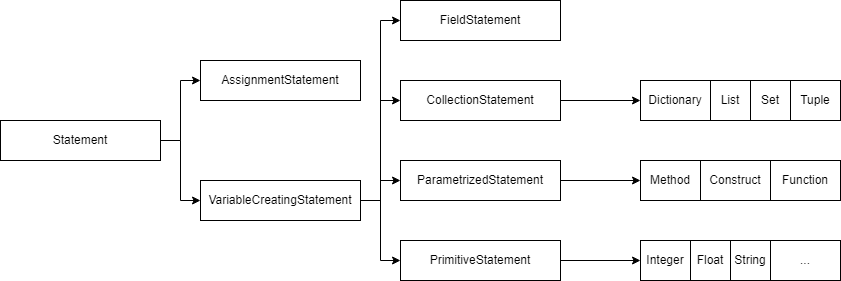
\includegraphics[width=1\textwidth]{Figures/statement_hierarchy2.png}
  \vspace*{0.5cm}
  \caption{Hierarchy of the \classname{Statement} class.}
\end{figure}

One class that assures Pynguin's easiness at the time of expanding it, is the abstract class \classname{GenerationAlgorithm}, which works as a layout for the insertion of any new heuristic of algorithm into the tool's current options, for the generation of \classname{TestSuiteChromosome}, another class wrapper for a list of \classname{TestCaseChromosome}.

In the context of evolutionary and genetic algorithms, the \classname{Statement} class has an abstract method called \callable{mutate}, which depending on the instance's final class, mutates either the primitive value, or the references that are encapsulated in it.

About the available algorithms\footnote{The work by Campos et al.~\cite{DBLP:journals/infsof/CamposGAFEA18} offers a further review and analysis of the different algorithms available in Pynguin.}, Pynguin has a total of 7: Random, Random Test Case Search, Random Test Suite Search, Whole Suite, MIO, MOSA and DynaMOSA.\@
From these, the experimental phase considered the last 4, because those implement either an archive or a dynamic chromosome population, which is necessary for the extension.

\begin{figure}[tb]
  \centering
  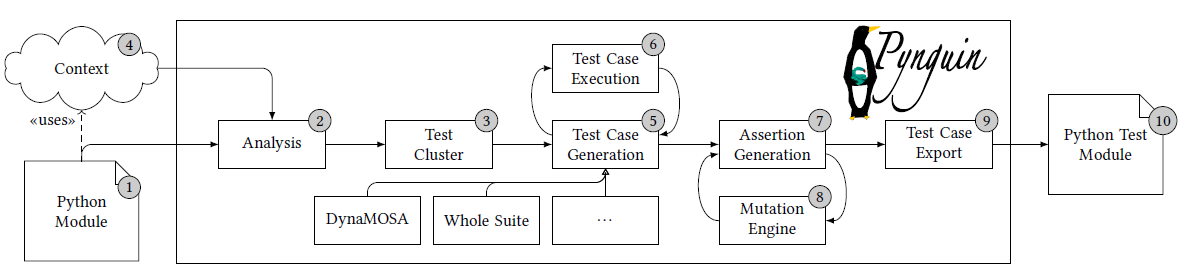
\includegraphics[width=.99\textwidth]{Figures/pynguin.png}
  \caption{Pynguin structure~\cite{DBLP:conf/icse/LukasczykF22}}\label{fig:pyn}
\end{figure}

Pynguin's workflow structure is presented in Figure~\ref{fig:pyn} and consists of a sequence of processes, starting with a Python Module as input, and getting a Python Test Module as output.
A general Pynguin execution begins by statically analysing the MUT in order to fill a ``Test Cluster'' with all relevant information for the posterior test generation, such as regarding types and methods.
Then, Pynguin individually picks functions or methods from the Test Cluster in order to generate a population (depending on the algorithm) of the \classname{TestCaseChromosome} class, firstly by generating a certain amount of either primitive, collection or instance statement used as parameter arguments, and then by generating the respective callable, owner of the different branches or lines to cover.
Once the final test suite is set, Pynguin tries to generate assertions for its test cases while creating mutations for themselves with MuyPY, to then export the final tests into new modules.

Pynguin also offers post generation processes, such as the deletion of redundant references (non-used variables) at the Chromosome level, or the generation of coverages reports for the output test files and spreadsheets with relevant information about the test generation, in HTML and CSV format respectively.

\newpage
\subsection{MOSA}

The Many-Objective Sorting Algorithm~\cite{DBLP:conf/icst/PanichellaKT15} (MOSA), is an improvement to the classic Multi-objective Optimization algorithms (MOA) such as the Non-dominated Sorting Genetic Algorithm II (NSGA-II) or the Strength Pareto Evolutionary Algorithm (SPEA2), and applied taking into account some specific draw backs of the branch coverage problem in test generation, such as the great computational effort needed by these classic algorithms when working with a number of objectives bigger than an order of magnitude of 10.
Another challenge that MOSA can overcome, is the selection and persistence over a non-dominated sort of those tests that have the best branch distance regarding non-covered goals.

Algorithm~\ref{alg:MOSApseudo} shows an overview of MOSA's pseudocode, which start with the generation of an initial random population.
Then, in every iteration an offspring is computed by means of arbitrary selection, crossover and mutation methods, which later is sorted into Pareto frontiers using Preference Sorting.
This procedure sets into the first frontier the best tests according to a preference criterion (usually the desired coverage), and then realizes a common Fast Non-dominated Sort over the rest of tests.
Finally, MOSA finishes every iteration of itself filling the next population with the right amount of tests from all the available Pareto frontiers.
About the MOSA implementation in Pynguin, it follows the same structure as the one in Algorithm~\ref{alg:MOSApseudo}.

\algrenewcommand\algorithmicrequire{\textbf{Input}}
\algrenewcommand\algorithmicensure{\textbf{Output}}


\begin{algorithm}[h!]
  \centering
  \caption{MOSA Pseudocode}\label{alg:MOSApseudo}
  \begin{algorithmic}[1]
    \Require~Stopping condition \(C\), Set of program targets \(B\), Population size \(M\)
    \Ensure~A test suite \(T\)
    \State~\(A, P_t \gets \{\}, \text{GenerateRandomPopulation}()\) 
    \While{\(\neg C\)}
      \State~\(Q_t \gets \text{GenerateOffspring}(P_t)\)
      \State~\(\text{UpdateArchive}(A, P_{t+1})\)
      \State~\(R_t \gets P_t \cup Q_t\)
      \State~\(F_x \gets \text{PreferenceSorting}(R_t)\)
      \State~\(P_{t+1} \gets \emptyset \)
      \State~\(d \gets 0\)
      \While{\(|P_{t+1}| + |F_d| \leq M\)}
        \State~\(\text{CrowdingDistanceAssignment}(F_d)\)
        \State~\(P_{t+1} \gets P_{t+1} \cup F_d\)
        \State~\(d \gets d + 1\)
      \EndWhile\@
      \State~\(\text{CrowdingDistanceSort}(F_d)\)
      \State~\(P_{t+1} \gets P_{t+1} \cup F_d[1\: (M - |P_{t+1}|)]\)
    \EndWhile\@
  \end{algorithmic}
\end{algorithm}

\newpage

\subsection{DynaMOSA}\label{sec:dynamosa}

DynaMOSA comes as a further extension of MOSA by Panichella et al.~\cite{DBLP:journals/tse/PanichellaKT18}, with the addition of a dynamic selection of the targets to be included into the first Pareto Frontier when executing the preference sorting.
The idea of including a dynamic selection of targets starts from the representation of a program into a CFG.\@
With it, is possible to note how those uncovered targets that have one or more already reached target predecessor are redundant to try to cover, because they always have objective score of \(f_r = \text{BranchDistance}(b) + 1\), where (\(+1\)) represents the approach level or the distance in the CFG to reach the successive target.
This means that every target can be prioritized into a hierarchy according to the definition of a CDG.\@

The pseudocode of DynaMOSA is shown in Algorithm~\ref{alg:DynaMOSApseudo}, with the only differences to MOSA being found in the lines 1, 5 and 9 when calling the set of an initial set of non-dependant targets and the dynamic update of these.
The \(\text{UpdateTarget}()\) procedure, is applied inside Pynguin by implementing a class for, a Control Flow Graph (named \classname{CFG}), as a wrapper of the \classname{ControlFlowGraph} class from the Python \classname{bytecode} module; and a Control Dependence Graph (called \classname{ControlDependenceGraph}).
Both of these classes are a fundamental part for the proposed heuristic implementation.

\begin{algorithm}[h!]
  \centering
  \caption{DynaMOSA Pseudocode}\label{alg:DynaMOSApseudo}
  \begin{algorithmic}[1]
    \Require~Stopping condition \(C\), Set of program targets \(B\), Population size \(M\), Control dependence graph \(G\), \(\phi\)~Map between edges of \(G\) and targets
    \Ensure~A test suite \(T\)
    \State~\(U^* \gets \text{NonDependentTargets}(B)\)
    \State~\(A, P_t \gets \{\}, \text{GenerateRandomPopulation}()\)
    \State~\(\text{UpdateTargets}(U^*, G, \phi)\)
    \While{\(\neg C\)}
      \State~\(Q_t \gets \text{GenerateOffspring}(P_t)\)
      \State~\(\text{UpdateArchive}(A, P_{t+1})\)
      \State~\(\text{UpdateTargets}(U^*, G, \phi)\)
      \State~\(R_t \gets P_t \cup Q_t\)
      \State~\(F_x \gets \text{PreferenceSorting}(R_t)\)
      \State~\(P_{t+1}, d \gets \emptyset, 0\)
      \While{\(|P_{t+1}| + |F_d| \leq M\)}
        \State~\(\text{CrowdingDistanceAssignment}(F_d)\)
        \State~\(P_{t+1} \gets P_{t+1} \cup F_d; d++\)
      \EndWhile\@
      \State~\(\text{CrowdingDistanceSort}(F_d)\)
      \State~\(P_{t+1} \gets P_{t+1} \cup F_d[1\: (M - |P_{t+1}|)]\)
    \EndWhile\@
  \end{algorithmic}
\end{algorithm}

\newpage

\subsection{Whole Test Suite}

The Whole Test Suite generation algorithm is an instance of a genetic algorithm that, as a result of custom operators, tries to optimize the computational effort of target coverage by evolving a population of test suites in a higher level of abstraction, compared to the other reviewed algorithms so far.
One of the main problems at the time of approaching test generation as a set of individual goals, is the case of encountering unreachable guards due to their recognition being an undecidable problem, and therefore it is not possible for the algorithm at hand to filter these elements in a trivial way.

Besides the preferred code coverage as fitness function, which is evaluated by running all test cases in a test suite and adding up all covered targets and distances, a secondary fitness function used is the size of the test suite, specifically for the forwarding of offspring chromosomes to further generations.
Algorithm~\ref{alg:WTSpseudo} shows Whole Test Suite's pseudocode, whose first relevant place is line 7 holding the crossover operator, that chooses a random value \(\alpha \in [0.0, 1.0]\) and generates 2 test suite offspring from the selected parents by splitting them both at position \(\alpha \times \text{Length}(p)\) and interchanging the segments.
Line 11 locates the mutation operator, where the algorithm mutates both test suites and test cases with a probability inverse to their own size, meaning that statistically only one of each are mutated in every iteration.
For test suites, with probability \(\sigma\) a new test case is added iteratively until the mutation fails.
Concurrently for test cases, three mutations can be applied with probability \(\frac{1}{3}\) each; remove, change or insert a statement.
The final novelty from this algorithm between lines 12 and 27, is the mechanism of generational forwarding already mentioned, which basically intends to bring the offspring to the next iteration's population only if either it has better fitness value, or if the fitness is equal to the one from the parents and the size of the offspring is much smaller.

In terms of the Whole Test Suite generation algorithm's implementation in Pynguin, it was done by setting a field in the \classname{WholeSuiteAlgorithm} class called \field{\_population}, containing a list of \classname{TestSuiteChromosome} objects.

\newpage

\begin{algorithm}[h!]
  \centering
  \caption{Whole Test Suite Pseudocode}\label{alg:WTSpseudo}
  \begin{algorithmic}[1]
    \Require~Stopping condition \(C\), Crossover probability \(P_c\)
    \Ensure~A test suite \(T\)
    \State~\(S \gets \text{GenerateRandomPopulation}()\)
    \While{\(\neg C\)}
      \State~\(Z \gets \text{Elitism}(S)\)
      \While{\(|Z| \neq |S|\)}
        \State~\(p_1,\, p_2 \gets \text{ParentRankSelection}(S)\)
        \If{\(P_c > \text{RandomFloat}()\)}
          \State~\(o_1,\, o_2 \gets \text{Crossover}(p_1,\, p_2)\)
        \Else\@
          \State~\(o_1,\, o_2 \gets p_1,\, p_2\)
        \EndIf\@
        \State~\(\text{Mutate}(o_1,\, o_2)\)
        \State~\(f_p \gets \text{MinimumFitness}(p_1,\, p_2)\)
        \State~\(f_o \gets \text{MinimumFitness}(o_1,\, o_2)\)
        \State~\(l_p \gets \text{Length}(p_1) + \text{Length}(p_2)\)
        \State~\(l_0 \gets \text{Length}(o_1) + \text{Length}(o_2)\)
        \State~\(T \gets \text{BestIndividual}(S)\)
        \If{\(f_o < f_p \lor (f_o = f_p \land l_o \leq l_p)\)}
          \For{\(o \in {o_1, o_2}\)}
            \If{\(\text{Length}(o) \leq 2\times \text{Length}(T)\)}
              \State~\(Z \gets Z \cup {o}\)
            \Else\@
              \State~\(Z \gets Z \cup {p_1 \text{or} p_2}\)
            \EndIf\@
          \EndFor\@
        \Else\@
          \State~\(Z \gets Z \cup {p_1, p_2}\)
        \EndIf\@
      \EndWhile\@
      \State~\(S \gets Z\)
    \EndWhile\@
  \end{algorithmic}
\end{algorithm}

\newpage

\subsection{MIO}

The Many Independent Objective (MIO) algorithm~\cite{DBLP:journals/infsof/Arcuri18} consists of a modification of the default (1 + 1) evolutionary algorithm, whose author came up with by taking the most notable characteristics of both MOSA and Whole Test Suite, in terms of exploration and exploitation of the search landscape.

One of these limitations, is the presence of a fixed size population that may not be big enough depending on the size of the System Under Test (SUT), the number of objectives to cover, or would not work optimally if too many redundant test have been introduced into it.
To fix this, MIO maintains an archive of test populations per target and sets a maximum amount of tests to be introduced to it.

MIO's core behaviour is represented by the existence of 3 main parameters; \(n\), being the number of tests per target to be stored in the archive; \(P_r\), the probability of introducing a randomly generated test into the population; and \(m\), the maximum amount of mutations to be applied.
To these, the algorithm also adds a fourth parameter \(F\), whose main purpose is to split the stopping conditions' budget in order to have two main phases with different sets of \(n\), \(P_r\) and \(m\).
Within the three parameters, it is stated that the first two are the more relatives ones at the time of controlling the exploration/exploitation.\@

A pseudocode of MIO is presented in Algorithm~\ref{alg:MIOpseudo}, which compared to Pynguin's implementation, only differs from the original algorithm's idea in the integrations of both \(T\) and \(A\) into a single data structure.

\begin{algorithm}[h!]
  \centering
  \caption{MIO Pseudocode}\label{alg:MIOpseudo}
  \begin{algorithmic}[1]
    \Require~Stopping condition \(C\), Population size limit \(n\), Start~of~focused search \(F\)
    \Ensure~Archive of optimized individuals A
    \State~\(T, A \gets \text{SetOfEmptyPopulations}(), \{\}\)
    \While{\(\neg C\)}
      \If{\(P_r > \text{RandomFloat}() \text{or IsEmpty}(T)\)}
        \State~\(p \gets \text{RandomIndividual}()\)
      \Else\@
        \State~\(p \gets \text{Mutate}(\text{SampleIndividual}(T))\)
      \EndIf\@
      \ForAll{\(k \in \text{ReachedTargets}(p)\)}
        \If{\(\text{IsTargetCovered}(k)\)}
          \State~\(\text{UpdateArchive}(A, p)\)
          \State~\(T \gets T \setminus \{T_k\}\)
        \Else\@
          \State~\(T_k \gets T_k \cup \{p\}\)
          \If{\(|T_k| > n\)}
          \State~\(\text{RemoveWorstTest}(T_k)\)
          \EndIf\@
        \EndIf\@
      \EndFor\@
      \State~\(\text{UpdateParameters}(F, P_r, n, m)\)
    \EndWhile\@
  \end{algorithmic}
  \end{algorithm} 

\newpage

\section{GBOS Heuristic}

The Graph Based Object Synthesis heuristic is the name given to the methodology presented by Yun et al.~\cite{DBLP:conf/sigsoft/0001O00D21} for the generation of complex object instances to be used as arguments in methods to be tested in a test case of the Java programming language.
One of the motivations for this research study was the possible non-continuity of test cases' search space with respect to coverage, when some related targets have the need to evaluate multiple conditions on an object instances before even getting an actual distance to them.
% TODO - maybe reference the example in the introduction?
The procedure done by this heuristic, consists of two main phases; the creation of an Object Construction Graph (OCG), that represents all relevant dependency flows of a method from its inputs to the actual target to be reached; and the translation of the OCG into an actual test case template, that serves as an initial search point for the test generation algorithm.

\subsection{OCG Generation}\label{subsec:ocg_gen}

For the generation of the OCG, one must start with the generation of the Program Dependency Graph (PDG), a complete representation of all control and data dependencies of a program.
As stated in Section~\ref{sec:slicing}, all dependencies of a program are represented with the aforementioned CDG and DDG.\@

The necessary PDG for the OCG's building process must also be interprocedural until a certain threshold level \(t_{\text{dep}}\), considering that one or many of the target method's input objects may be modified by a subsequent call.
This new requirement is met by just adding to the main PDG new edges from the correspondent callee's basic block to the entry node of the other method or function PDG, which also needs to be generated beforehand.

After having the full interprocedural PDG, a node containing a branch \(b\) (chosen target for the heuristic) must be used as entry criteria to apply a backward slice and either a node with an instruction reading a method input, a node with an instruction reading a global variable or an entry node, as stopping criteria.

The following step, is to analyse the sliced graph and link directly every instance of a node loading the complex method parameter objects with any node from the interprocedural methods' PDGs that retrieve a field or access an array, so the relevant variable state of these objects can be recorded flawlessly throughout the graph.

Finally, the sliced PDG is sliced further in a forward manner, using the object method inputs as slicing criteria and any field or array access as stopping condition, in order to leave only relevant paths for the heuristic's second phase.

\subsection{OCG Translation}

Once the OCG generation process is complete, its translation into actual code is done by including extra operations to a generic Breadth-first graph traversing algorithm.
The first step, is to initialize a test case \(t\) with a call to the target branch's method (and its respective object in case it is not static) together with an empty node-statement map.
Then, every time a relevant node is reached, such as the ones containing instructions of parameter loading, or attribute/array accessing, a corresponding object creating statement or attribute setting mechanism is added into the test and saved in the node-statement map.
The only case in which a field is called with a getter instead of a setter, is when the correspondent node is not a leaf, because this means that there might be a successor node either containing an array access or getting an object type field.
The purpose of the previously mentioned map, is to have direct reference of any object input at the time of setting its fields.

Considering the static typing of Java, one last matter to take in mind is the setting of non-public and non-static fields, which have to be managed through appropriate getter or setter methods.
This procedure is done by analysing all possible methods \(M = {m_1, m_2, \dots, m_k} \) in the correspondent class and building a directed call graph between them with paths \(P = \langle m_s, \dots, m_e\rangle\), where \(p_s\) represents the starting method, \(p_e\) the exit method that finally sets the field and the rest, the methods in between.
Using these two definitions, it is possible to approximate the likelihood of every method to set the field correctly with a metric composed of the number of parameters \(N_v\) and the complexity of the path \(P\).
For computing the path complexity, it is also necessary to check for every node in the path, what the ration between branches \(B'\) that access the next node in the path versus the total branches \(B\) is.
The path score is given by the equation
\begin{equation*}
  \text{score}(P) = (N_v + 1)\left(\frac{\sum_{s}^{e} \frac{|B'|}{|B|}}{|P|}\right)
\end{equation*}
and the sampling probability of a method \(m_i\) can be calculated by normalizing the maximum path score of every path that contains \(m_i\).

\chapter{GBOS Pynguin Extension}\label{chap:implementation}

Part of the preparations for the experimental phase and contributions of this thesis, is the creation of a functional extension of Pynguin inspired in the GBOS heuristic, that had to be developed using only the information available in its respective paper~\cite{DBLP:conf/sigsoft/0001O00D21} and some hints given by the authors of it.
The presented Python implementation followed a three-step scheme at Python Bytecode level, which aimed to be as loyal as possible to the original Java version while taking into account the differences between both languages.

\section{PDG Generation}

The development process started with the creation of \classname{DataDependenceGraph}, a new subclass of the already implemented \classname{ProgramGraph}, which serves as a superclass for both (also already available) \classname{CFG} and \classname{ControlFlowGraph}.
As its name hints, this new graph class encapsulates all necessary methods and further elements that help to collect all relevant data usages and definitions for the later generation of the reaching definitions sets.
Another crucial information obtained with the generation of the DDG through this class, are the methods and functions called along the program's control flow.  

In a first instance, one of the prerequisites for the coding of a DDG in Pynguin, was to split every node's basic block in the CFG class, into nodes with singular instruction.
If this had not been done, the final DDG would have set many variable uses and definitions in the same basic block node, simplifying the final graph to a trivial level that would have not worked in the further steps of the heuristic.
An example of this is shown in Figure~\ref{fig:ddg_example}.

\begin{figure}[htb]
  
\end{figure}

\begin{figure}[htb]
  \minipage{0.3\textwidth}
    \inputminted{python}{Figures/basic_block.py}
  \endminipage\hfill
  \minipage{0.65\textwidth}
    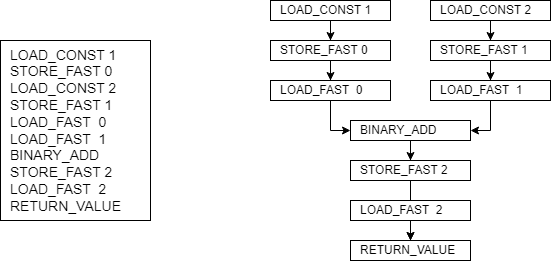
\includegraphics[width=\textwidth]{Figures/DDG.png}
  \endminipage\hfill
  \caption{A function \callable{foo} (left), a DDG of the function generated from a basic block CFG (middle) and another DDG, but generated from a single instruction CFG (right).}\label{fig:ddg_example}
\end{figure}


Then, the program's stack frame evolution is statically simulated and analysed to check which nodes have an instruction that defines or uses any variable names, or what functions or methods are called.
Opposite to off-the-shelf implementations of a stack frame analyser for Java (e.g. Java ASM\footnote{https://asm.ow2.io}), the used and defined data variables were collected every time they were either popped and served as operand for an instruction (e.g. BINARY\_ADD), and stored in the named stack or loaded back again in the stack frame (e.g. STORE\_FAST or LOAD\_FAST). 
This functionality was put into practice thanks to the classes \classname{DefUseAnalyzer} and \classname{Frame}, that traverse the CFG in a breadth-first manner and execute the corresponding single instruction respectively.

The way this works in the method \callable{DefUseAnalyzer.analyse}, is that every entry node starts with an empty \classname{Frame} with no variables in its stack.
Then, each non-entry node copies the frame from the first of its successors, execute the current instruction (with the method \callable{Frame.execute}) and set this modified copy as its own.
All the instructions' stack effects can be found in Python's developer documentation\footnote{https://docs.python.org/3.10/library/dis.html}.
As a design decision, the GBOS heuristic works with the bytecode instructions of Python version 3.10, because: it is one of Pynguin's supported versions; it restricts the amount Python Bytecode instructions needed to be implemented in the stack modifying match-case statement found in the \callable{Frame.execute} method; and it is stated in the GBOS paper~\cite{DBLP:conf/sigsoft/0001O00D21} that the approach is ``applicable in more general cases'', which implies the heuristic to work in any level of abstraction.

% TODO - Add an example of how frame works. method is called execute()

Once the \classname{DefUseAnalyzer} finishes generating two dictionaries (node, [variables]) for the uses and definitions, the DDG generation procedure copies every node in the given CFG, and proceeds to traverse once again the CFG in a breadth-first manner to apply the reaching definitions equations presented in Section~\ref{sec:slicing} to obtain the edges of the new graph.

With a program's DDG already generated, the CDG is obtained with the already implemented methods to do so, and the previously modified single-instruction CFG.\@
Both of these graphs are the base of the computation of an instance of the class \classname{ProgramDependenceGraph}, another subclass of \classname{ProgramGraph}, that initially just combines the edges of both CDG and DDG.\@
A second procedure realized as part of the PDG's computation, is the use of Pynguin test cluster and the (node, callable) dictionary obtained while getting the stack frame information, for the computation of subsequent called methods' PDGs.
This is done in a recursive manner and complying to a certain recursion level \(t_{\text{dep}}\), that works as a newly introduced Pynguin CLI argument. 

At this point, the interprocedural PDG is ready to be backward sliced with the necessary stopping conditions, contextualized to Python's bytecode instructions.
The slicing begins with the single instruction node in the PDG that contains the target branch, and it stops when either the node loads one of the target method's parameters (e.g.\@it is the first LOAD\_FAST that has one of the target method's parameters as argument) or it has a LOAD\_ATTR instruction; the node has a LOAD\_GLOBAL instruction; or the node has no predecessors (it is an entry node).

\section{PDG Interprocedural Analysis}\label{sec:pdgia}

The interprocedural analysis is the next step to follow, and it starts by iterating over the list of know calls and selecting only the methods to check for the presence of an instruction chain 
\[\begin{pmatrix} \text{LOAD\_FAST} \\ \text{or} \\ \text{LOAD\_ATTR} \\ \text{or} \\ \text{BINARY\_SUBSCR} \end{pmatrix} \rightarrow \text{LOAD\_METHOD} \rightarrow \text{CALL\_METHOD}\]
that represents the load of the object instance, the load of its method and the call of it.
Within the scope of the current study, the analysis of function type callables (not belonging to any object or class definition) is left as a recommended future work subject, considering that working with a dynamically typed language is already challenging when applying a heuristic designed for a statically typed language (such as Java) and that there is not a reliable way of knowing how to link the arguments of a called function (probably loaded before a LOAD\_FUNCTION instruction) to their respective local variables inside the sub graph of the interprocedural PDG.\@

Then, from the first instruction node of the chain (that represents the callee of the method), it is needed to look into the sub-PDG of the called method for the first ``LOAD\_FAST self'', which represents the same object instance and might have a successor node LOAD\_ATTR that needs to be linked to the first node in the initial chain.

Figures~\ref{fig:inter_analysis} represents the outcome of an interprocedural analysis applied to the OCG of the method \callable{checkRules} from Listing~\ref{lst:1}.
There, the section marked as ``Interprocedural PDG'' corresponds to the sub-PDG of the method \callable{getActor} which is called at the node ``CALL\_METHOD 0''.
What the analysis does here, is replacing the method call edge into a direct data-dependency edge between ``LOAD\_FAST action'' (parameter input object) and ``LOAD\_ATTR \_actor'' (object field).

\begin{figure}[htb]
  \minipage{0.49\textwidth}
    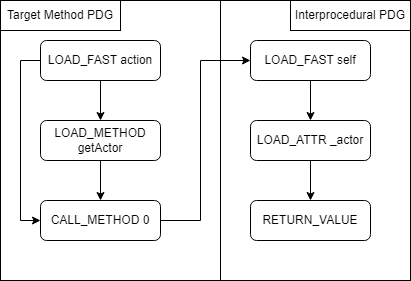
\includegraphics[width=\linewidth]{Figures/before_analysis.png}
  \endminipage\hfill
  \minipage{0.49\textwidth}
    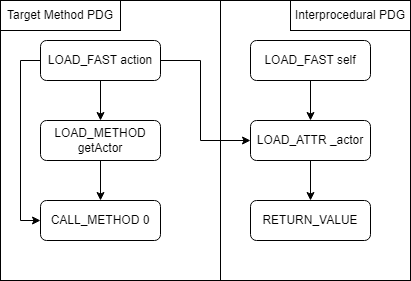
\includegraphics[width=\linewidth]{Figures/after_analysis.png}
  \endminipage\hfill
\caption{An example of OCG before and after the interprocedural analysis}\label{fig:inter_analysis}
\end{figure}

A forward slicing is then performed into the PDG, starting from the parameter loading nodes and stopping at relevant nodes (those with LOAD\_ATTR or BINARY\_SUBSRC instructions) fulfilling certain conditions.
The conditions for this operation are, that the relevant nodes stop the slicing, if and only if they do not have any more child nodes that are also relevant.

To give a comparative of the OCG creation process between Lin et al.'s Java implementation~\cite{DBLP:conf/sigsoft/0001O00D21} and the one from this thesis, Figure~\ref{fig:ocgs} shows both the OCG previous to the forward slicing from the original paper of the heuristic, and the OCG generated with Pynguin and its extension.

\begin{sidewaysfigure}[bhtp]
  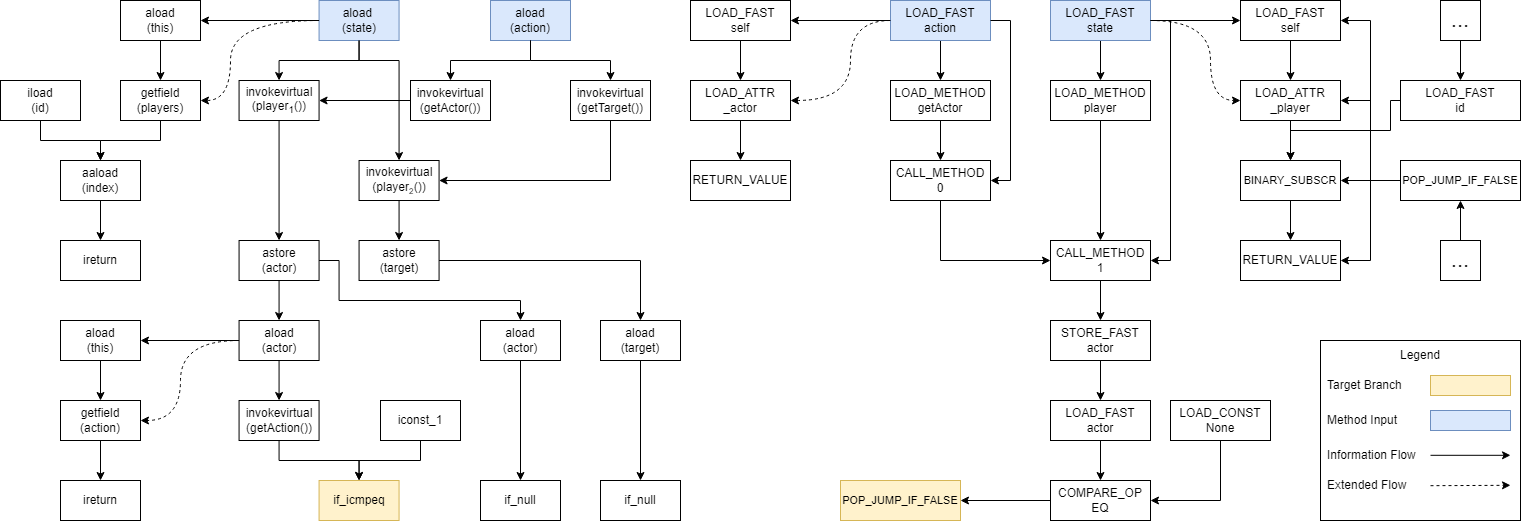
\includegraphics[width=\textwidth]{Figures/ocg_graphs.png}
  \caption{On the left, a representation of the OCG generated from the work of Lin et al.~\cite{DBLP:conf/sigsoft/0001O00D21}, and on the right, an OCG for the parallel target branch, when executing Pynguin with the GBOS extension.}\label{fig:ocgs}
\end{sidewaysfigure}

\section{OCG Translation}

When the OCG generation phase is ready, the last step of the GBOS heuristic is to translate it, in this case, into a \classname{TestCaseChromosome} instance.
The creation of it begins with a default empty chromosome, to which two possible main statements are added: a call statement of the target method or function, and positioned before that, a variable creating statement with the class containing that method.
This last statement is ignored if the target callable is a function.

Before starting to generate statements, the target method is analysed one more time, using Python's AST\footnote{https://docs.python.org/3.10/library/ast.html} and Astroid\footnote{https://pylint.pycqa.org/projects/astroid/en/latest/} libraries, in the look for any useful type annotation that might be inside the \classname{FunctionDef} and \classname{ClassDef} of the target method's module AST.\@ 
Then, similar to most of the previous graph traversing steps, the OCG is covered in a breadth-first manner while maintaining an (ID,~variable~reference) map to keep track of all the created object instances and set fields.
The keys of the map are set to ID = parentID~+~'.'~+~instruction.arg, with the idea  to avoid redundancy at the time of adding statements to the test case.
An example of this, is the possible appearance of a node with the instruction ``LOAD\_FAST state'' multiple times within the OCG, which could lead to generating multiple object instances of type \classname{GameState} even though it is necessary to generate it only once.
This implies, that only a variable reference is stored in the map for the key ``state'' at the first appearance of ``LOAD\_FAST state'', or for the key ``state.\_players'' at the first appearance of the chain ``LOAD\_FAST state \(\rightarrow\) LOAD\_ATTR \_player''.

Although the OCG was sliced thoroughly during its generation, most  of the nodes in it are still irrelevant for statement creation.
This, because at this point the only instructions that are interesting for the test case template are those that load object instances such as the ones from method's inputs, load attributes of the aforementioned object inputs, and access possible collection-like data types from Python, which might have further complex objects as elements.

For nodes that encapsulate a \textbf{LOAD\_FAST} instruction, an object instance is created in case the node's argument is one of the target method's parameters, and it is the first appearance of it.

With \textbf{LOAD\_ATTR} nodes, first it is checked if there is any existent key in the variable reference map regarding one of the current node's predecessors. 
If there is an already created object instance, an assignment statement is added into the test case, with a field access of the object as the left-hand side of the assignment, and a new primitive or object variable reference as the right-hand side.
Regarding the path score, used to select the adequate setter method in the heuristic's paper Java implementation, there was no need to apply it in this Python version, as Python does not have an applied concept of private fields.
At most, there is the developer community standard of using an underscore (``\_'') character before a field variable name to simulate it as private, but this does not have any real run-time implications.
One argument for implementing a non-arbitrary way to select a certain method to set fields, is that there is not a concrete way in the actual Python's literature, to know if a method modifies a certain field, other than the presence of the instructions LOAD\_ATTR, STORE\_ATTR or DELETE\_ATTR.\@
The usage of getters in the original Java version was replaced in this case with the variable reference map, which provides information regarding the position of the object instance inside the test case, the type information and the annotations, if available.
Overall, this is the main and only difference between this thesis' work and the original heuristic proposed by Lin et al.~\cite{DBLP:conf/sigsoft/0001O00D21}.

When encountering a \textbf{BINARY\_SUBSRC} instruction, the OCG is checked to look for a predecessor node with an already generated collection variable that contains object elements.
In both ``LOAD\_FAST'' and ``LOAD\_ATTR'', the list variables are initialized with a few references of the same variable as elements (1 to 10, as arbitrary values), and when these are object types, the used instance is the one stored into the map of references.
In this context, this node only takes any available reference of the parent nodes, but as it needs to save it every time to start the chain of references, the index of this node in the reference map is the string version of its own index.

Once the test case template generation process is finished, the test case is executed with the available \classname{TestExecutor} instance, and the results are stored into the same \classname{TestCaseChromosome}.
Listing~\ref{lst:6} presents one of the cases generated when using the GBOS extension, showing particular similarity with the hypothetical test template proposed in Listing~\ref{lst:4}.

\begin{figure}
  \inputminted[linenos]{python}{Figures/template-result.py}
  \caption{Mutated test template obtained through the execution of Pynguin with the GBOS extension for the test of the example module in Listing~\ref{lst:1}\label{lst:6}}
\end{figure}

For every extended algorithm, the following steps are done

\begin{itemize}
  \item MIO:\@ the archive is updated with the implemented method of the archive instance \callable[\text{test\_template}]{MIOAlgorithm.\_archive.update}.

  \item MOSA and DynaMOSA:\@ the test template is first checked for any execution exception and then introduced into the '\_population' field of the \classname{AbstractMOSAAlgorithm} class, which is a list of \classname{TestCaseChromosome} elements.
  \item Whole Test Suite: same as for MOSA and DynaMOSA, the test template is checked for exceptions and then is introduced in one of the \classname{TestSuiteChromosome} available in the '\_population' field of the algorithm instance, \classname{WholeSuiteAlgorithm}.
\end{itemize}

About the new parameters introduced to Pynguin for the GBOS heuristic, there is the binary argument ``gbos'', meaning the usage of the extension; the numerical argument ``no\_change\_iteration'', stating the amount of iteration in which there may be no change in a certain goal in order to consider it eligible to create a new test template for; the float argument ``p\_app'', describing the probability of creating a test template for an eligible target; and the numerical argument ``max\_recursion\_level'', defining the maximum amount of recursion calls that can be made while generating the OCG.\@

One remark that must be taking into account with respect to the implementation, is that the GBOS extension relies completely on the assumption that the any time a complex object input is needed for the reaching of a branch target, all required type information about the parameters and relevant object fields will be available. 

\chapter{Evaluation}~\label{chap:evaluation}

The previous work on the implemented GBOS extension has shown that in a general case, using this heuristic improved significantly the coverage results of automatically generated tests of Java classes.
In the same way, it is relevant to study the behaviour of Pynguin's GBOS implementation in terms of coverage, while analysing the programming style of the Python modules of the testing set.
Therefore, the following research questions are formulated:

\begin{resq}
  Can the Graph-Based Object Synthesis extension outperform Pynguin in its original paper's experimental setup similarly as EvoObj did with EvoSuite?
\end{resq}

For the answer of this Research Question, a union of two previous test sets of Pynguin's research papers was put to the test to benchmark the performances of both Pynguin in the latest developer version (0.35.0) that the repository had before cloning it and the extension to the tool, presented by this thesis.
To avoid redundancy in the results, from the total amount of modules, only those that are not considered trivial stayed for the evaluation (more details about the test set in Section~\ref{sec:experimental_setup}).
Then, from the branch coverage results, a Mann-Whitney U test and the Cohen D's effect size measure were calculated in order to compare them to the results obtained by Yun Lin et al. 

\begin{resq}
  Is there a correlation between the difference in coverage results and the amount of object-like callable inputs of MUTs while using Pynguin and the GBOS extension?
\end{resq}

In this scenario, the same module set from the previous research question was used.
From the test set, the percentage of object-like inputs in methods and functions was obtained by analysing the AST of the MUTs with the following formula
\begin{equation}\label{eq:olr}
\text{OLR} = \frac{1}{n}\sum_{m_i \in M} \frac{o_i}{p_i}
\end{equation}
where \(M\) is the set of callables in a MUT with at least one object-like parameter, \(p_i\) the amount of parameters in \(m_i\), \(o_i\) the amount of object-like parameters in \(m_i\), and \(n\) the amount of methods in \(M\) (from now on, the metric is called the object-like ratio or OLR).
An object-like parameter references any method argument that has type information, and it is not either one of Python's primitive types or built-in collections.
One exception to this rationale, is when one argument is identified as a collection type that has object-like types as elements which, although it could be considered a recursive rule, it was limited to a first class wrapper.
Here, the OLR serves as a way to imply the presence of complex object inputs and see if the metric presents a correlation with the development of branch coverage when using or not the extension.
For those modules that stay in the test set for this research question after a filtering process, the \(\hat{A}_{12}\) Vargha-Delaney effect size metric is going to be computed in order to calculate the Pearson's and Spearman's correlation, and answer the research question. 

\section{Experimental Setup}\label{sec:experimental_setup}

For the experimental executions of Pynguin with the new GBOS extension, the data set of Python projects initially used as a benchmark for Pynguin's type tracing update, joined with a subset of Pynguin's EMSE submission test modules~\cite{DBLP:journals/corr/abs-2111-05003}, was taken as a base for the answer of both research questions.
This initial testing set is formed by 1047 modules over 44 projects.

In a first instance, are going to be filtered all modules that reach full branch coverage using the MIO algorithm without the GBOS extension, before 100 iterations or 600 seconds of execution search time.
The filtering process left at this point 588 modules over the same 44 projects.
For the answering of the second research question, a final filtering criteria was applied by comparing the  results of the runs to their Import Coverage, and checking the object-like ratio described in Equation~\ref{eq:olr}.
Here, only those modules that have a final coverage that is different to their Import Coverage value or have a OLR greater than \(0.5\) are kept.
In the run statistical data set there were some configurations of module and approach that did not reach more than 10 runs, and were also removed from the following analysis.

Regarding the execution parameters of Pynguin, 8 main configurations are used to cover the 4 extended algorithms, and either the usage or not usage of the GBOS extension itself.
The configurations that used the WHOLE\_SUITE argument, needed additionally to set the parameter ``--use\_archive'' to true, as the extension uses the archive of each \classname{GenerationAlgorithm} to obtain the branch goals.
From the newly introduced parameters, only ``--no\_change\_iterations'' was tuned in a hand-made manner while having the first test runs as reference.
In these (and similar to the results finally used for the analysis), the runs using the MIO algorithm reached mean algorithm iteration values close to an order of magnitude between \(10^5\) and \(10^6\), contrary to the rest of algorithms, which reached values closer to an order of magnitude of \(10^4\).
Because of this, the mentioned parameter was left at the default value of \(1000\) for MIO, and lowered to \(300\) for the other algorithms.
The maximum execution time was set to 600 seconds, and the remaining parameters were set to Pynguin's default values, as no further Parameter Tuning was applied.

As a way to make visible the possible execution time trade-off between the different phases of the GBOS extension and Pynguin's own search time output value, and apply the subsequent analysis individually, new output variables were introduced into the post-search process.
These are ``GBOSDecisionTime'' and ``GBOSGenerationTime'', representing the amount of time the GBOS extension needed for checking if the conditions to entering the generation phase were met, and for the test template generation phase itself, respectively.
In that sense, the time measure stored in the new variables is not counted as part of the already implemented ``SearchTime'', but are part of ``TotalTime''.

\section{Threats to Validity}

The threats to validity present in the study can be generalized into two main categories: threats to \textbf{internal validity}, to \textbf{external validity} and to \textbf{construct validity}.

The GBOS extension's \textbf{internal validity} is threatened by the uncertainty of how many possible cases of what is considered a complex callable input are covered, including the amount of recursions in wrapper classes that are taking into account while computing the type annotations, or the consideration of all wrapper classes available for Python in its 3.10 version.
The definition of the Object-like ratio also makes an internal threat, as it was used as an intermediary step into identifying the possible complex object inputs, stating that primitive types axiomatically are not objects nor complex, but at the same time it is not a determinant measurement.
An example of this is a variation of the method \callable[]{checkRules} from Figure~\ref{lst:1}, but taken from line 1 until before line 10, where the method would have an OLR of \(100\%\) but the unique target (branch of line 8) would not need any complex object in order to be reached.
The plausible presence of bugs in the multiple stages of the GBOS phase also threatens the internal validity, which is partially mitigated by the if-clauses that stop the whole process if one of the steps returns a None value (e.g.\ while constructing the PDG, OCG or the test template).
The necessity of both complex object inputs and full knowledge of the variables' type information in order to obtain any improvement in terms of branch coverage threatens the internal validity too.

With respect to the generalization of the benefits obtained from the presented extension, the \textbf{external validity} is threatened by the usage of Python modules that were already studied in previous studies of Pynguin, and might not represent the great majority of Python modules. 

About \textbf{construct validity}, the usage of the extension cannot be decided through Parameter Tuning, but only via the knowledge of each developer of the presence of complex object inputs in a method or function, which implies that no automatic tuning was made into the experimental phase, threatening the study's operationalization.


\section{Research Question 1}

\begin{figure}[b]
  \minipage{0.5\textwidth}
    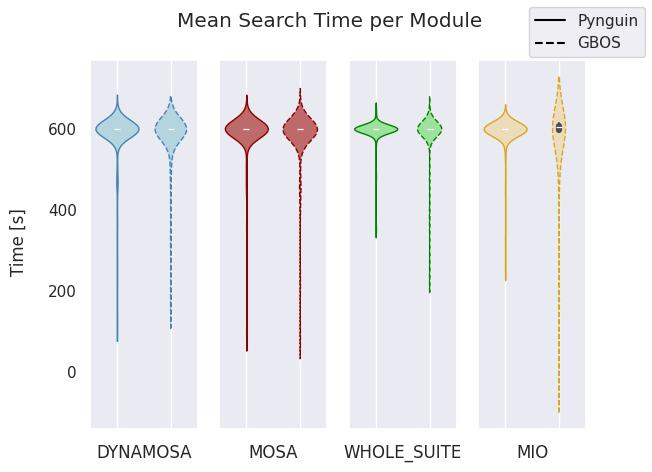
\includegraphics[width=\linewidth]{Figures/Results/SearchTime.jpg}
  \endminipage\hfill
  \minipage{0.5\textwidth}
    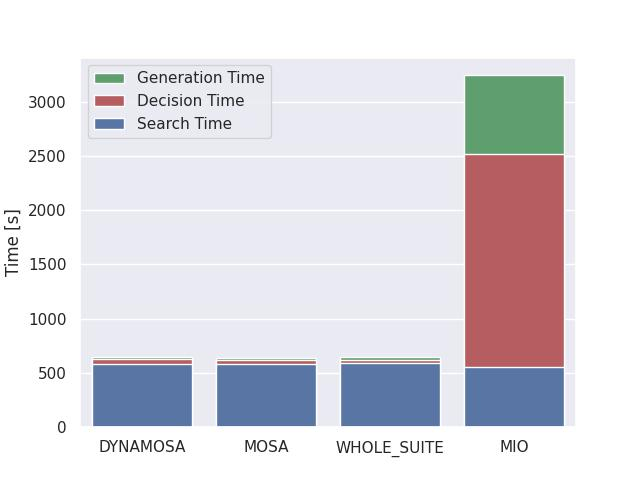
\includegraphics[width=\linewidth]{Figures/Results/timeDist.jpg}
  \endminipage\@
  \caption{Search time distribution between the 8 parameter configurations and average values for new output variables of the GBOS extension.}\label{fig:times}
\end{figure}

Figure~\ref{fig:times} describes through two plots the overall search time and the time needed by the extension per phase.
For these plots, only were accounted those modules that had valid results in the 8 configurations at the same time.
The violin plot on the left, shows the Search Time distribution of the runs, revealing that both Pynguin and the extension use the full budget of 600 seconds for any computation that is not related to the GBOS extension.
The percentage change (e.g.~\(\frac{\text{GBOSValue} - \text{PynguinValue}}{\text{PynguinValue}}\times 100\)) for the average values of the distributions presented in this plot are \(\SearchTimeDYNAMOSA\), \(\SearchTimeMOSA\), \(\SearchTimeWHOLESUITE\) and \(\SearchTimeMIO\) respectively, from left to right.

Regarding the times that are considered while doing any GBOS-related operation, the bar plot on the right shows a comparison of the average values per module, per algorithm, of the time spent in deciding if the current iteration generates a test template or not (Decision Time), time spent generating the test templates (Generation Time), and the Search Time as baseline.
By looking at the sizes of the different sections of each algorithms' bars, it is safe to state that compared to the other options, MIO is the algorithm that is affected the most with the extra computational effort that the GBOS extension generates.
This can be explained by the lightweight nature of the evolution steps implemented in Pynguin, which are reduced to only selecting a new test case if necessary and mutating it the maximum amount of times possible depending on the algorithm's parameters.
Considering a comparison between the Search Time and the Decision Time, MIO obtains a percentage change of \(\DiffDecMIO\), while the other algorithms have values ranging between \(\DiffDecMin\) and \(\DiffDecMax\).
With respect to the Generation Time, the comparison using percentage change of MIO gives a value of \(\DiffGenMIO\), while the other algorithms have values ranging between \(\DiffGenMin\) and \(\DiffGenMax\).

The data reported in Table~\ref{tab:performance} shows the mean coverage of all tested modules per approach, the p-Values obtained through statistical Mann-Whitney U tests and Cohen's D effect size measures, in any pair of algorithm and runtime budget.
Generally, all p-Values are greater than \(0.05\) with respect to the sets of obtained branch coverage values in each module, accepting the null hypothesis that assumes no effect or statistical difference between the distributions.
Complementary, Figure~\ref{fig:coverage} shows the branch coverage results and their distribution through the runs of the 8 different parameter configurations.
The presented violin plots imply that in general, both approaches to the test generation for the set of Python modules got similar results, based on the form of the plots' probability density, the position of the median and the position of the interquartile range.

\begin{figure}[tbh]
  \centering
  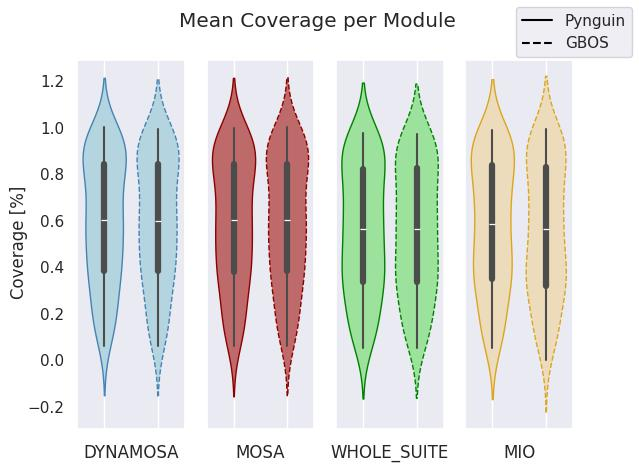
\includegraphics[width=0.9\textwidth]{Figures/Results/Coverage.jpg}
  \caption{Mean coverage between all 8 parameter configurations over the modules in the test set.}\label{fig:coverage}
\end{figure}

Nonetheless, it is noticeable that all values of Cohen's D effect size in Table~\ref{tab:performance} are negative, meaning that the best distributions of coverage values are found while using Pynguin without the GBOS extension.
This strongly implies that in a general Python developing scenario the usage of the GBOS extension is not advised nor makes any considerable improvement in coverage results, as the mean effect size found in the last time step budget of the runs gets a value of \(\AverageCohen\) over all algorithms, contrary to the value of \(0.21\) (in favour of EvoObj) obtained by Yun Lin et al.\ over all the algorithms used in their experimental phase for the maximum budget of 300 seconds. 

\begin{table}[h!]
  \centering
  \begin{tabular}{lcccc}\toprule 
\multirow{2}{*}{Coverage Performance} & \multicolumn{4}{c}{Budget - 300[s] } \\ \cmidrule(lr){2-5}  
                                      & DYNAMOSA&MOSA&WHOLESUITE&MIO                         \\ \midrule 
GBOS                                  & \(0.62\)&\(0.62\)&\(0.62\)&\(0.61\)                       \\ 
Pynguin                               & \(0.62\)&\(0.62\)&\(0.62\)&\(0.62\)                       \\ 
p Value                               & \(1.0\)&\(1.0\)&\(0.98\)&\(0.93\)                     \\ 
Cohen's D Effect Size                 & \(0.01\)&\(0.01\)&\(-0.01\)&\(-0.2\)                       \\ 
\bottomrule 
\end{tabular}
  \centering
  \begin{tabular}{lcccc}\toprule 
\multirow{2}{*}{Coverage Performance} & \multicolumn{4}{c}{Budget - 450[s] } \\ \cmidrule(lr){2-5}  
                                      & DYNAMOSA&MOSA&WHOLESUITE&MIO                         \\ \midrule 
GBOS                                  & \(0.6\)&\(0.6\)&\(0.57\)&\(0.59\)                       \\ 
Pynguin                               & \(0.61\)&\(0.61\)&\(0.57\)&\(0.61\)                       \\ 
p Value                               & \(0.75\)&\(0.76\)&\(0.71\)&\(0.76\)                     \\ 
Cohen's D Effect Size                 & \(-0.25\)&\(-0.2\)&\(-0.26\)&\(-0.51\)                       \\ 
\bottomrule 
\end{tabular}
  \centering
  \begin{tabular}{lcccc}\toprule 
\multirow{2}{*}{Coverage Performance} & \multicolumn{4}{c}{Budget - 600} \\ \cmidrule(lr){2-5}  
                                      & DYNAMOSA&MOSA&WHOLESUITE&MIO                         \\ \midrule 
GBOS                                  & \(0.59\)&\(0.59\)&\(0.56\)&\(0.5\)                       \\ 
Pynguin                               & \(0.61\)&\(0.6\)&\(0.58\)&\(0.59\)                       \\ 
p Value                               & \(0.69\)&\(0.69\)&\(0.67\)&\(0.43\)                     \\ 
Cohen's D Effect Size                 & \(-0.62\)&\(-0.47\)&\(-0.46\)&\(-4.77e+12\)                       \\ 
\bottomrule 
\end{tabular}
  \caption{Coverage Performance of Pynguin and GBOS with different time budgets.}\label{tab:performance}
\end{table}

A summary of the amount of modules used in every step of this research question is found in Table~\ref{tab:modrq1}, including the initial set before the filtering of those configurations that did not reach 10 runs, and after the intersection of modules between those available for both main approaches (default Pynguin and GBOS).

\begin{table}[t]
  \centering
  
\begin{tabular}{lcccc}\toprule
    \multicolumn{1}{c}{\multirow{2}{*}{\# Modules}} & \multicolumn{4}{c}{Pynguin}                \\ \cmidrule(lr){2-5}
    \multicolumn{1}{c}{}                          & DynaMOSA & MOSA    & WHOLE SUITE & MIO     \\ \midrule
    Initial Set                                     & \(557\)  & \(553\) & \(555\)     & \(551\) \\
    RQ1 Before Intersection                         & \(541\)  & \(540\) & \(544\)     & \(538\) \\
    RQ1 After Intersection                          & \(109\)  & \(109\) & \(109\)     & \(109\) \\ 
    \bottomrule
  \end{tabular}
  \centering 
  \begin{tabular}{lcccc}\toprule
    \multicolumn{1}{c}{\multirow{2}{*}{\# Modules}} & \multicolumn{4}{c}{GBOS}                   \\ \cmidrule(lr){2-5}
    \multicolumn{1}{c}{}                          & DynaMOSA & MOSA    & WHOLE SUITE & MIO     \\ \midrule
    Initial Set                                     & \(553\)  & \(554\) & \(555\)     & \(527\) \\
    RQ1 Before Intersection                         & \(529\)  & \(523\) & \(539\)     & \(118\) \\
    RQ1 After Intersection                          & \(109\)  & \(109\) & \(109\)     & \(109\) \\ 
    \bottomrule
\end{tabular}

\caption{Amount of modules used while analysing each experimental configuration  for the answering of Research Question 1.}\label{tab:modrq1}
\end{table}


\begin{summary}{RQ1: Performance of GBOS over Pynguin}
  The presented GBOS extension for Pynguin \textbf{does not} outperform Pynguin itself while being evaluated over previously studied modules, similarly as EvoObj outperformed EvoSuite. 
\end{summary}

\newpage

\subsection*{Discussion}

With the results in Table~\ref{tab:performance}, it is shown once more how the extra computational effort needed while using the GBOS extension does not influence the obtained coverage results, at least as a rule of thumb.
One possible factor that explains the lack of improvement, is the absence of a need for complex object inputs by the modules under test in order to reach all target branches (which will be exemplified later).
This latter argument can be backed up partially with the results in Figure~\ref{fig:times}, which tell that even after the applied filtering, some modules still could reach a full branch coverage with the tests provided by an initial population of test chromosomes (e.g.~getting a Search Time of 0 [sec]).
In addition, the data per time budget step mostly says that during the coverage evolution of Pynguin using MIO, there is a slightly bigger difference in performance while using the extension, which can be attributed to the random nature of the Search Based algorithms, or to the inter-iteration time difference in the Search Time variable when using the extension, in the case of the final time step of 600 seconds.

Figure~\ref{fig:best} shows the branch coverage evolution along the 600 seconds budget for those modules that obtained the best effect size values on each algorithm.
In these, during the whole search time budget it can be remarked how both curves have the same results, following the behaviour already found in Table~\ref{tab:performance}.
This can be backed by the number of runs successfully executed, as all of these modules had at most 10 runs of difference between both the main approaches.

\begin{figure}[ptbh]
  \centering
  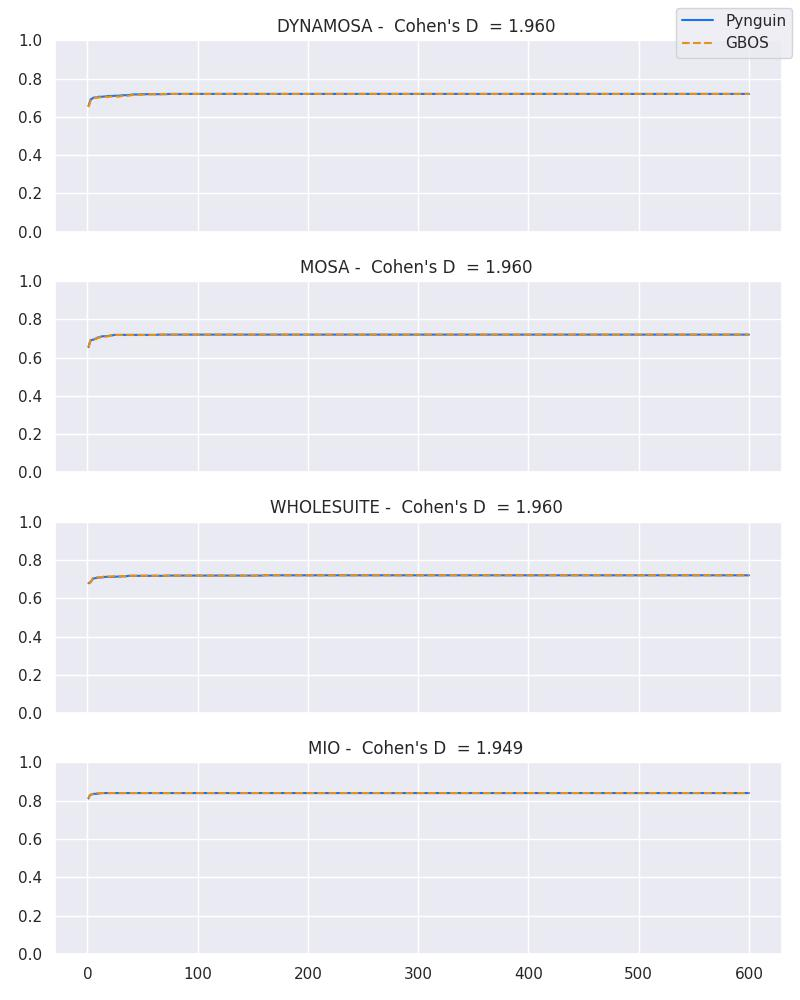
\includegraphics[width=0.9\textwidth]{Figures/Results/bestES.jpg}
  \caption{Branch coverage evolution for the modules that obtained the best Cohen's D effect size value in each algorithm.}\label{fig:best}
\end{figure}

Although these graphs imply that the heuristic did not have any positive effect in the coverage results, this statement is not conclusive, as all the p-Values presented in Table~\ref{tab:performance} invalidate the statistical difference between both distributions.
Taking this into account, the different information logs provided by Pynguin during the test template generation process were gathered in order to understand the general behaviour over the modules.
Table~\ref{tab:flag_modules} shows the amount of modules in each one of the algorithms, that followed a certain scenario while using the GBOS heuristic.
From the 588 original modules, the different sets that could be recognized are; those that had at least one correct run; those that had at least one log from the heuristic, and thus, started it; those that managed to create a non-empty template within their evolution process; those that created a template that brought no execution errors, and was added into the population; those that did not start a generation process because they had no branch coverage goals to choose from; and those that finished their execution early, because of a Pynguin-related runtime error (e.g.~a thread had to be killed, the maximum recursion depth was met, or the exception ``Bug in Pinguin'' was raised). 


\begin{table}[t]
  \centering
  
\begin{tabular}{lcccc}\toprule
    \multicolumn{1}{c}{\# Modules that}    & DynaMOSA   & MOSA      & WHOLE SUITE   & MIO     \\ \midrule
    had correct runs                               & \(553\)  & \(554\) & \(555\)     & \(527\) \\
    had logs from the heuristic                    & \(399\)  & \(393\) & \(402\)     & \(423\) \\
    created a template                             & \(348\)  & \(342\) & \(357\)    & \(355\) \\ 
    added a template                               & \(347\)  & \(340\) & \(352\)    & \(353\) \\ 
    had no coverage goals                          & \(35\)  & \(35\) & \(26\)    & \(52\) \\ 
    had runtime errors                             & \(15\)  & \(20\) & \(13\)    & \(42\) \\ 
    \bottomrule
  \end{tabular}

\caption{Sizes of the different relevant module groups gathered from the set of runs provided by the GBOS extension.}\label{tab:flag_modules}
\end{table}

At this point, the last two types of relevant modules would be those that either: got an increase in coverage, defying the current no improvement conclusions; or got a similar coverage result, but in fewer algorithm iterations.
With these in mind, ``setuptools.command.setopt'' and ``slugify.\_\_main\_\_'' are for each case the best modules respectively, with an improvement of \(0.066\) points in branch coverage, and a reduction of \(-99.587\%\) in the amount of iterations, while executing the extension with DynaMOSA and MIO.\@

Nonetheless, both of these modules have no type annotations regarding any class with attributes, nor any if-else guard that uses any complex object (see Listing~\ref{lst:8}) as most of the boolean values are comparisons of strings, or collections keys.
Another found case can be shown in Listing~\ref{lst:7}, where the function \callable[]{edit\_config} needs (implicitly) the paths to already created files, which goes over the capabilities of the heuristic.

This would imply that the improvement in coverage was given by the chosen Pynguin seeds, and the reduction in iteration number obtained by the longer iteration time caused the added steps of the heuristic (decision and generation), together with a convergence of coverage in the early evolution of the runs.

\begin{figure}
\begin{minted}[highlightlines={8, 11, 12, 16, 19, 24, 30}]{python}
  # Module setuptools.command.setopt
  def edit_config(filename, settings, dry_run=False):
    log.debug("Reading configuration from %s", filename)
    opts = configparser.RawConfigParser()
    opts.optionxform = lambda x: x
    opts.read([filename])
    for section, options in settings.items():
        if options is None:
            log.info("Deleting section [%s] from %s", section, filename)
            opts.remove_section(section)
        else:
            if not opts.has_section(section):
                log.debug("Adding new section [%s] to %s", section, filename)
                opts.add_section(section)
            for option, value in options.items():
                if value is None:
                    log.debug("Deleting %s.%s from %s", section, option, filename)
                    opts.remove_option(section, option)
                    if not opts.options(section):
                        log.info(
                            "Deleting empty [%s] section from %s", section, filename
                        )
                        opts.remove_section(section)
                else:
                    log.debug(
                        "Setting %s.%s to %r in %s", section, option, value, filename
                    )
                    opts.set(section, option, value)
    log.info("Writing %s", filename)
    if not dry_run:
        with open(filename, 'w') as f:
            opts.write(f)
\end{minted}
\caption{Example of methods from the module setuptools.command.setopt, with highlighted branches.}\label{lst:7}
\end{figure}

\begin{figure}
\begin{minted}[highlightlines={5, 7, 10, 14, 16, 18}]{python}
  # Module slugify.__main__
  def parse_args(argv: list[str]) -> argparse.Namespace:
    parser = argparse.ArgumentParser(description="Slug string")
    # Intermediary code
    if args.input_string and args.stdin:
        parser.error("Input strings and --stdin cannot work together")
    if args.replacements:
        def split_check(repl):
            SEP = '->'
            if SEP not in repl:
                parser.error("Replacements must be of the form: ORIGINAL{SEP}REPLACED".format(SEP=SEP))
            return repl.split(SEP, 1)
        args.replacements = [split_check(repl) for repl in args.replacements]
    if args.input_string:
        args.input_string = " ".join(args.input_string)
    elif args.stdin:
        args.input_string = sys.stdin.read()
    if not args.input_string:
        args.input_string = ''
    return args
\end{minted}
\caption{Example method from the module slugify.\_\_main\_\_, with highlighted branches.}\label{lst:8}
\end{figure}

Listing~\ref{lst:9} presents examples of test templates generated (but not necessarly used) by the heuristic when working over the module setuptools.command.setopt, which focused on the method \callable[]{config\_file}.
In this case, the only branches available are evaluated by comparing strings.

\begin{figure}
\begin{minted}[highlightlines={}]{python}
import setuptools.command.setopt as module_0
'''
def config_file(kind="local"):
    if kind == 'local':
        return 'setup.cfg'
    if kind == 'global':
        return os.path.join(os.path.dirname(distutils.__file__), 'distutils.cfg')
    if kind == 'user':
        dot = os.name == 'posix' and '.' or ''
        return os.path.expanduser(convert_path("~/%spydistutils.cfg" % dot))
    raise ValueError("config_file() type must be 'local', 'global', or 'user'", kind)
'''
def test_case_0():
    dict_0 = dict()
    any_0 = module_0.config_file(dict_0)

def test_case_1():
    float_0 = -2881.7
    any_0 = module_0.config_file(float_0)

def test_case_2():
    str_0 = "'Vq.2 -oz+)-@l"
    any_0 = module_0.config_file(str_0)
\end{minted}
\caption{Example of test templates generated by the heuristic for the module setuptools.command.setopt}\label{lst:9}
\end{figure}

On the other side, the test templates synthesized for slugify.\_\_main\_\_ were only empty ones, when trying to cover the branch present in the snippet

\begin{minted}{python}
if __name__ == '__main__':  # pragma: no cover
  main()
\end{minted}

at the end of the module.

\newpage

\section{Research Question 2}

Figure~\ref{fig:scatter} shows a scatter plot of the different modules that presented an OLR measure greater than \(50\%\) and their Vargha-Delaney \(\hat{A}_{12}\) effect size with respect with the two distributions available for each approach and algorithm.
For each graph, modules that had valid runs while using both Pynguin and the extension were taken into account, leaving an amount of modules between \(\MinMod\) and \(\MaxMod\) after the OLR filtering.
In this figure, the general effect size average over all algorithms is given by the value \(\AverageA\). 

\begin{figure}[bth]
  \centering
  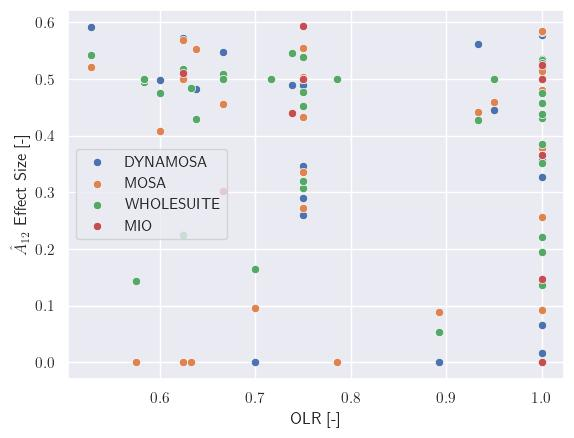
\includegraphics[width=0.9\textwidth]{Figures/Results/scatterplot.jpg}
  \caption{Scatter plot of the \(\hat{A}_{12}\) effect size values versus the OLR value, for every module that reported a OLR value greater than \(0.5\)}\label{fig:scatter}
\end{figure}

To answer this research question, two types of correlations metrics were calculated; Pearson's correlation coefficient, for linear dependency; and Spearman's rank correlation coefficient, for monotonic relationship between the variables.
Both of these metrics are categorized depending on the magnitude and sign of their values, ranging from \(-1\) to \(1\) and stating a strong correlation for magnitudes closer to \(1\), a direct relation for positive values and an inverse relation for negative values.

The values obtained for each metric follow a repetitive behaviour in each algorithm; the Pearson's correlation coefficient values ranged between \(\MinPearson\) and \(\MaxPearson\), meaning mostly no linear correlation between the variables OLR and \(\hat{A}_{12}\) effect size; the Spearman's rank correlation coefficient values ranged between \(\MinSpearmans\) and \(\MaxSpearmans\), meaning no monotonic correlation between the variables OLR and \(\hat{A}_{12}\) effect size; implying, that there is no correlation (or a weak correlation) between the aforementioned variables, when using the GBOS extension in a general Python module scenario.
One could infer a possible linear correlation when applying MIO, as it got a Pearson correlation greater than 0.5, but considering the gathered data this far from the previous research question, this values is not conclusive.

A summary of the amount of modules used in every step of this research question is shown in Table~\ref{tab:modrq2}, including once again the initial module set before the filtering of those configurations that did not reach 10 runs, the preliminary filter of the modules that reached a coverage result greater than the import coverage, and the posterior intersection of modules, which included only those modules that have an OLR greater than \(50\%\).

\begin{table}[t]
  \centering
  
\begin{tabular}{lcccc}\toprule
    \multicolumn{1}{c}{\multirow{2}{*}{\# Modules}} & \multicolumn{4}{c}{Pynguin}                \\ \cmidrule(lr){2-5}
    \multicolumn{1}{c}{}                          & DynaMOSA & MOSA    & WHOLE SUITE & MIO     \\ \midrule
    Initial Set                                     & \(557\)  & \(553\) & \(555\)     & \(551\) \\
    RQ2 Before Intersection                         & \(492\)  & \(490\) & \(494\)     & \(487\) \\
    RQ2 After Intersection                          & \(43\)  & \(42\) & \(46\)     & \(9\) \\ 
    \bottomrule
  \end{tabular}
  \centering 
  \begin{tabular}{lcccc}\toprule
    \multicolumn{1}{c}{\multirow{2}{*}{\# Modules}} & \multicolumn{4}{c}{GBOS}                   \\ \cmidrule(lr){2-5}
    \multicolumn{1}{c}{}                          & DynaMOSA & MOSA    & WHOLE SUITE & MIO     \\ \midrule
    Initial Set                                     & \(553\)  & \(554\) & \(555\)     & \(527\) \\
    RQ2 Before Intersection                         & \(479\)  & \(472\) & \(489\)     & \(115\) \\
    RQ2 After Intersection                          & \(43\)  & \(42\) & \(46\)     & \(9\) \\ 
    \bottomrule
\end{tabular}

\caption{Amount of modules used while analysing each experimental configuration for the answering of Research Question 2.}\label{tab:modrq2}
\end{table}

\begin{summary}{RQ2: Correlation of coverage improvement and OLR}
  The usage of the presented GBOS extension \textbf{does not} induce a correlated improvement in branch coverage results, when applied to Python modules that have a higher OLR metric.
\end{summary}

\subsection*{Discussion}

\begin{figure}[ptbh]
  \centering
  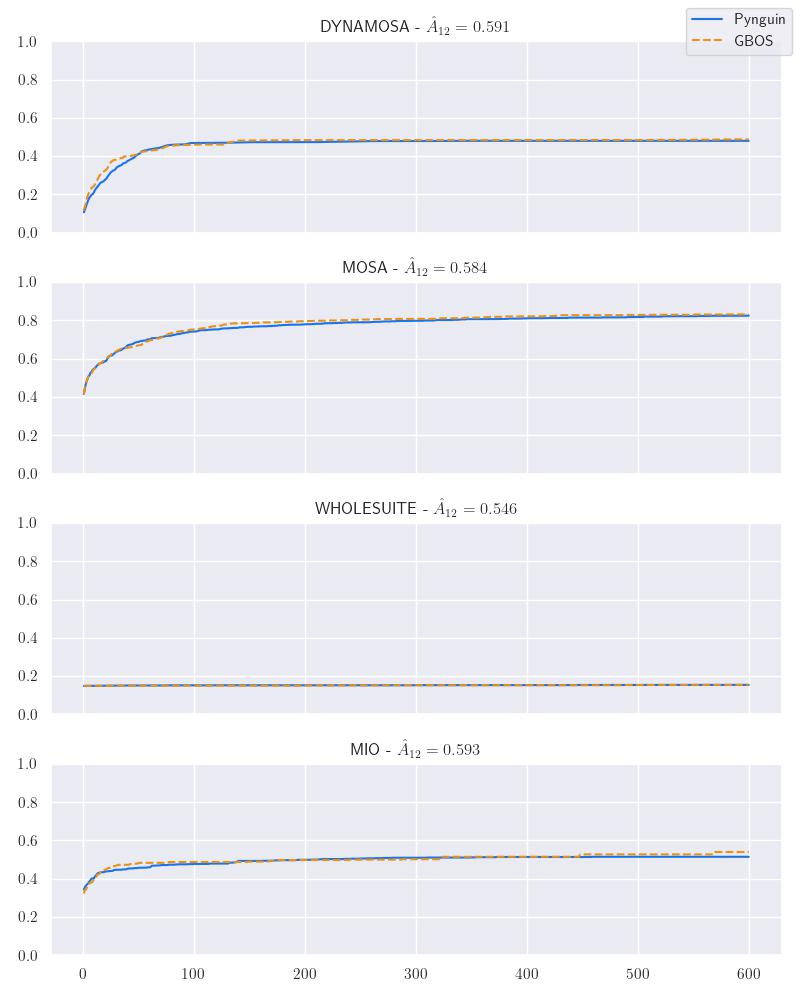
\includegraphics[width=0.9\textwidth]{Figures/Results/bestA12.jpg}
  \caption{Branch coverage evolution for the modules that obtained the best Vargha-Delaney \(\hat{A}_{12}\) effect size value in each algorithm.}\label{fig:besta12}
\end{figure}


The obtained answer for the second research question develops the same ideas as the discussion of the first research question, leaning to an initial tought, that the majority of Python modules in the testing set either, do not include enough type information or the necessity for complex object inputs. 
See Figure~\ref{fig:besta12} for a timeline of coverage for the modules that got the best \(\hat{A}_{12}\) values.

To test this theory, once again modules were analysed from the two relevant scenarios: those were the extension results got a coverage improvement, or reached the same results as Pynguin but in less algorithm iterations.
For these, the modules were ``pkg\_resources.\_vendor.jaraco.functools'', with an increase of \(0.047\) in coverage, and ``setuptools.\_vendor.importlib\_resources.\_legacy'', with a decrease of \(86.45\%\) in the number of computed iterations.
The two modules have an OLR value of \(0.75\) and \(0.78\) respectively.

Listing~\ref{lst:10} shows two out of the three present callables within the module ``pkg\_resources.\_vendor.jaraco.functools'' that influenced the given OLR value.
In them, the class CallableT is an alias of the built-in class CallableType from the typing library added in Python 3.5, that does not hold any attributes in its definition, nor need them for any branch.
This class is at the same time an alias for callables from the ``collections.abc'' module with two parameters. 

\begin{figure}
\begin{minted}[highlightlines={}]{python}
CallableT = TypeVar("CallableT", bound=Callable[..., object])
def method_cache(
    method: CallableT,
    cache_wrapper: Callable[
        [CallableT], CallableT
    ] = functools.lru_cache(),  # type: ignore[assignment]
) -> CallableT:
    def wrapper(self: object, *args: object, **kwargs: object) -> object:
        bound_method: CallableT = types.MethodType(  # type: ignore[assignment]
            method, self
        )
        cached_method = cache_wrapper(bound_method)
        setattr(self, method.__name__, cached_method)
        return cached_method(*args, **kwargs)
    wrapper.cache_clear = lambda: None  # type: ignore[attr-defined]

    return (  # type: ignore[return-value]
        _special_method_cache(method, cache_wrapper) or wrapper
    )
\end{minted}
\caption{Example method \callable[]{method\_cache} with non-primitive types parameters from the module pkg\_resources.\_vendor.jaraco.functools}\label{lst:10}
\end{figure}

For the next case, Listing~\ref{lst:11} presents three callables from the second relevant module with parameters of type \classname{Package} and \classname{Resource}, aliases of either a string or the ModuleType class.
These, together with the rest of modules that have any non-primitive type annotation on the signature, have no branches to cover.

\begin{figure}[thbp]
\begin{minted}[highlightlines={}]{python}
Package = Union[types.ModuleType, str]
Resource = str
def open_binary(package: Package, resource: Resource) -> BinaryIO:
    return (_common.files(package) / normalize_path(resource)).open('rb')
def read_binary(package: Package, resource: Resource) -> bytes:
    return (_common.files(package) / normalize_path(resource)).read_bytes()
def open_text(
    package: Package,
    resource: Resource,
    encoding: str = 'utf-8',
    errors: str = 'strict',
) -> TextIO:
    return (_common.files(package) / normalize_path(resource)).open(
        'r', encoding=encoding, errors=errors
    )
\end{minted}
\caption{Example functions that have type annotations detected as object-like by the heuristic from the module setuptools.\_vendor.importlib\_resources.\_legacy}\label{lst:11}
\end{figure}

As a final aspect, Figures~\ref{lst:12}~and~\ref{lst:13} display the test templates created for the two specific modules when using heuristic, which focus mainly in callables that do have a branch to cover, but do not expose any type information.
Similar to the already analysed case, this would imply that both ``improvements'' were not achieved by the heuristic.
For example, the idea of the extension focusing callables without type information and synthesizing simple test templates over pkg\_resources.\_vendor.jaraco.functools, makes the improvement in coverage be explained once again only by Pynguin's random nature.
Additionally, in the module with fewer iterations when using the extension rather than Pynguin, it happened that the test generation process had an unexpected error in the early stages while already getting the best coverage obtained by the default settings, thus ending the whole run earlier. 

\begin{figure}
\begin{minted}[highlightlines={}]{python}
import pkg_resources._vendor.jaraco.functools as module_0
'''
class Throttler:
    def __init__(self, func, max_rate=float('Inf')):
        if isinstance(func, Throttler):
            func = func.func
        self.func = func
        self.max_rate = max_rate
        self.reset()
def retry_call(func, cleanup=lambda: None, retries=0, trap=()):
    attempts = itertools.count() if retries == float('inf') else range(retries)
    for attempt in attempts:
        try:
            return func()
        except trap:
            cleanup()
    return func()
'''
def test_case_0():
    none_0 = None
    throtler_0 = module_0.Throttler(none_0, none_0)
def test_case_1():
    none_0 = None
    any_0 = module_0.retry_call(none_0, none_0)
\end{minted}
\caption{Example of test templates generated by the heuristic for the module pkg\_resources.\_vendor.jaraco.functools}\label{lst:12}
\end{figure}

\begin{figure}
\begin{minted}[highlightlines={}]{python}
import setuptools._vendor.importlib_resources._legacy as module_0
'''
def normalize_path(path: Any) -> str:
    str_path = str(path)
    parent, file_name = os.path.split(str_path)
    if parent:
        raise ValueError(f'{path!r} must be only a file name')
    return file_name
'''
def test_case_0():
    none_0 = None
    str_0 = module_0.normalize_path(none_0)
\end{minted}
\caption{Example of test templates generated by the heuristic for the module setuptools.\_vendor.importlib\_resources.\_legacy}\label{lst:13}
\end{figure}

\newpage

\section{Further Analysis}\label{sec:further}

To give a brief description of the different modules that made up the test set, Figure~\ref{fig:olr-hist} shows a ranged histogram (with bins of length \(0.1\)) of Object-like ratios over the 588 executed modules with the continuous line representing the kernel density estimate.
From these, \(91.33\%\) of the modules, or 537 out of 588 have a ratio below \(50\%\).
This values might explain the null improvement when using the GBOS extension, as one of the prerequisites to make the implemented heuristic work, is to have full type information regarding the possible complex object inputs needed to reach the target branches.
Analogously, the OLR distribution does not mean that for the great majority of modules there are not any needed complex object input, but that only for those that have an OLR greater than \(0.0\%\) (and by chance include a target reachable by generating a test with a complex object input) the presented GBOS may be of help in the improvement of coverage results.

\begin{figure}[bth]
  \centering
  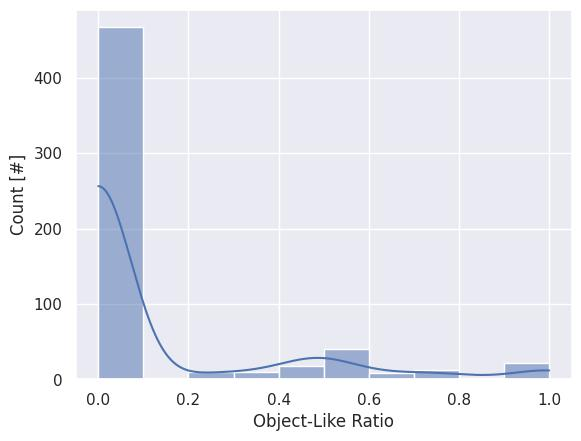
\includegraphics[width=0.9\textwidth]{Figures/Results/olr-hist.jpg}
  \caption{Histogram of Object-like ratio over the modules in the test set.}\label{fig:olr-hist}
\end{figure}

For a deeper understanding of the information logs that were introduced to Pynguin for the test template generation process, these mainly tried to check what steps of the test template generation were being reached during all tries.
The logs are added into a Python set if any of the following conditions are met at any point during the test suite generation:
\begin{itemize}
  \item a PDG, or a non-sliced OCG is created with or without errors
  \item either the backward slice, interprocedural analysis or forward slice were performed without errors
  \item a test template is (or not) generated
  \item a test template is (or not) added into the algorithm's population.
\end{itemize}
Besides, any message from a raised Exception that was not related to any of the previous points, was also added into the set.

With this information, it was possible to understand that for out \(90\%\) of the modules from the original test set that had a correct run, more than half of them created and added test templates into the population with no effect on the results. 
This fact can be explained by a lack of type information (which made the heuristic create trivial templates) or a lack of necessity for complex objects, and backs up the answers given to the proposed research questions.

An additional example of this behaviour is the module ``py\_backwards.compiler'', which obtained one of the best \(\hat{A}_{12}\) effect size values for DynaMOSA, but still did not find any coverage improvement.
The encountered phenomenon can be attributed to the difference in runs (9) and that the value was not high (0.591).

Further examination of this module, indicates that a class \classname{CompilationTarget} is imported and used as parameter in it (``target''), but is it only the alias for a Tuple of two integers.
This parameter is evaluated in a single guard.

\begin{minted}[highlightlines={1, 7}]{python}
def _transform(path: str, code: str, target: CompilationTarget) -> Tuple[str, List[str]]:
    debug(lambda: 'Compiling "{}"'.format(path))
    dependencies = []  # type: List[str]
    tree = ast.parse(code, path)
    debug(lambda: 'Initial ast:\n{}'.format(dump(tree)))
    for transformer in transformers:
        if transformer.target < target:
            debug(lambda: 'Skip transformer "{}"'.format(transformer.__name__))
            continue
        debug(lambda: 'Use transformer "{}"'.format(transformer.__name__))
        working_tree = deepcopy(tree)
        try:
            result = transformer.transform(working_tree)
        except:
            raise TransformationError(path, transformer,
                                      dump(tree), format_exc())
        if not result.tree_changed:
            debug(lambda: 'Tree not changed')
            continue
        # ... Branchless code ...
    return fix_code(code), dependencies
\end{minted}

Considering the current cases, were most of the modules did not have correct type annotations for the heuristic to work, or a need for complex objects for the heuristic to be usefull, questions arise about the precense of logs informing of POP operations to an empty stack when generating the DDG, which is most likely due to certain cases that could not be resolved completely in the implementation and might have caused a variable information loss.\@

One example of this is when the MUT has ``try-except'' or ``with'' clauses inside any of its basic blocks.
The problem with these logic rules comes, because their implementation is given (on the 3.10 Python version) with Python instruction that conditionalize the stack frame state on the presence of an Exception, e.g.~\textbf{SETUP\_WITH} and \textbf{SETUP\_FINALLY}.
An example of this behaviour is the snippet

\begin{minted}{python}
try:
    # A SETUP_FINALLY is emitted here, pointing to the except block
    pass
except:
    pass
\end{minted}

where the stack frame suffers no relative change in case of no Exception, or is restored to its state before the ``try'' block and pushes different Exception-related variables onto the stack (e.g.~the raised Exception, the address of the exception handler, etc.) before continuing in the ``except'' block on the contrary case.  
The procedure in this type of instruction for the development stage of the extension was to set the node's stack frame effect to be the one given by the successful execution.

With this case present in the OCG generation, it is non-trivial to obtain the use and definition places, and consequently it is not possible to fully define the reaching definition equations.
Nonetheless, a full control flow from the start of the callables to the return statements can still be found as a sub-graph within each CFG, meaning that it can still be possible to get the necessary instructions where variables are used or defined regarding the relevant ones.

Regarding once more the example module presented in Figure~\ref{lst:1}, the line plots shown in Figure~\ref{fig:example_cov} show the evolution in branch coverage results over a Search Budget of 600 seconds for four cases of two characteristics each, either using or not the GBOS extension, and either using MIO and MOSA as examples of evolutionary and genetic algorithms.
In them, it is remarkable how none of the baseline Pynguin approaches could escape the search landscape local optima, which is attributed to the random nature prevalent in both algorithms, together with the limited search time.
Contrastingly, both GBOS approaches reached the full coverage before spending the whole search time budget, when using ``no\_change\_iteration'' arguments of 100 and 500 for MOSA and MIO respectively.
These latter experimental instances show a better performance in terms of sooner convergence when using the MIO algorithm, which is explained by the fact that although MIO was configured to generate test templates less often compared to MOSA, previous results showed that the amount of iterations that MIO performs is exponentially greater to other algorithms.
Moreover, the way MIO is implemented into Pynguin makes the execution of it prioritize the mutation of each iteration's single solution, thing that is strictly necessary in order to reach branch targets after generating a test code template. 

\begin{figure}[htb]
  \centering
  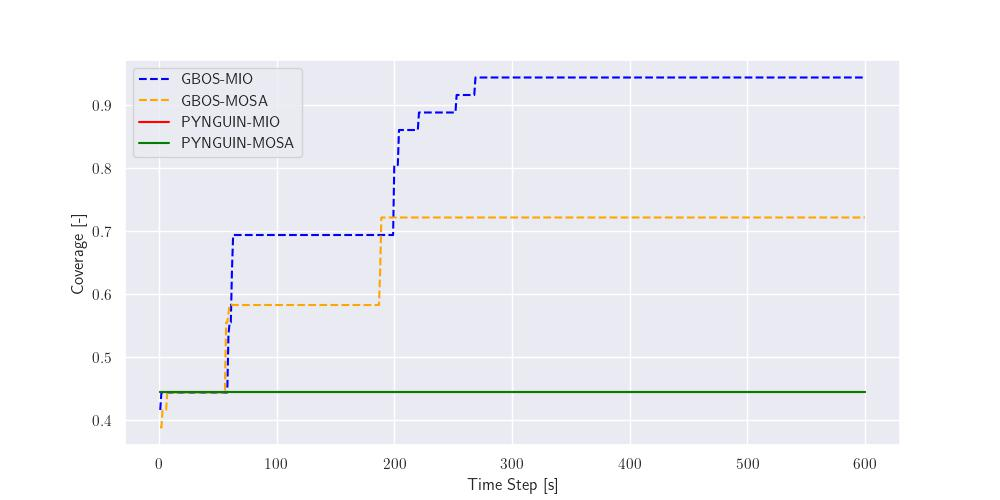
\includegraphics[width=0.9\textwidth]{Figures/Results/exampleCov.jpg}
  \caption{Coverage evolution while running Pynguin for the example module introduced in Chapter~\ref{chap:introduction}.}\label{fig:example_cov}
\end{figure}

\chapter{Related Work}\label{chap:related_work}

Before commenting on the different tools and techniques that have a place in the current state of the art of automatic test generation for programming languages, it is worth describing the types of testing and their objectives. Unit testing is a type of functional testing that tries to test individual or atomic units of a software project.
Regression testing, on another side, is a type of system testing that tells if new functionalities of a system produce defects into the latest build of it.

The various approaches that are part of the current state-of-the-art for Automatic Test Generation can be categorized in two main types depending on what are they based on: Large Language Models (LLMs) and Search-Based Algorithms or Static Analysis (SB).

\section{LLM-Based}

\subsection*{CodaMOSA}

One of the many tools presented in papers that have cited Pynguin in their research is CodaMOSA~\cite{DBLP:conf/icse/LemieuxILS23}, software created by Microsoft developers, has Pynguin as a base and extends its functionality calling OpenAI's Codex\footnote{https://openai.com/blog/openai-codex} API to get template suggestions for test cases that are in a coverage stall, similar to what this thesis works over.
For the development, the authors used only MOSA as the search algorithm because is the only one that allowed the usage of both line and branch coverage as fitness functions, on the version of Pynguin at the time (0.19.0).

The procedure done by CodaMOSA, queries prompts to Codex after the coverage has not changed in a certain amount of iterations, and from a set of target generations of chromosomes that it statistically chooses to generate a test from either a function, method or constructor.
After that, it deserializes the returned test case from Codex into the internal representation of Pynguin, while applying different heuristics, such as removing nested expressions and use single assignment.

For the benchmark, modules from 35 projects from the Pynguin paper were filtered so just those that do not fail to produce result and those that do not reach \(100\%\) coverage in less than a minute are experimented over.
The baselines for the experimental phase were Pynguin with MOSA and CodexOnly, which while being compared to CodaMOSA were statistically compared using the Mann-Whitney U-Test.
The results showed that CodaMOSA performs significantly better, reaching a higher coverage on 173 more modules compared to MOSA and 279 more modules compared to CodexOnly.

\subsection*{MutAP}

Mutation testing is one software testing technique, that aims to measure the ability of a test to reveal bugs.
Taking this approach in mind, Dakhel et al.\@ presented in 2023 MutAP~\cite{DBLP:journals/corr/abs-2308-16557}, another LLM based code generation tool that also introduces prompt augmentation for killing mutants in an iterative process before the actual synthesis of test cases.

\begin{figure}[tb]
  \centering 
  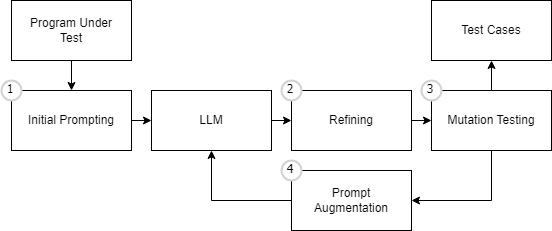
\includegraphics[width=.99\textwidth]{Figures/mutap.png}
  \caption{MutAP structure}\label{fig:mutap}
\end{figure}

A summary of MutAP's structure is shown in Figure~\ref{fig:mutap}, and after inputting a Python Program Under Test (PUT), it commences with the building of an initial prompt for the obtaining of an initial test case.
The first step (1), employs one of the two following learning methods; zero-shot, where the PUT is concatenated after the statement  ``Generate test case for the following code''; and few-shot, which concatenates the PUT after a sequence of pairs of a method and its respective unit test.
After the initial test is synthesized, the second step (2) consists of re-prompting it, so possible syntax errors can be corrected and unintended behaviour can be repaired.
Then, the third step (3) introduces mutations into the PUT using MutPy\footnote{https://pypi.org/project/MutPy/0.3.0/} so that the quality and effectiveness of the tests can be assessed.
At this point, the algorithm of MutAP has a conditional path depending on the number of surviving mutants; if there are none, the test cases are considered finished and generated; and in the contrary case, the prompt augmentation step is followed.
This post conditional step (4), adds information to a new prompt of the LLM, such as the already refined initial test, the statement ``The test function, \(\text{test}()\), cannot detect the fault in the
following code'', one of the mutant survivors, and a final statement ``Provide a new test case to detect the fault in prior code''.

In the experimental trial of this tool's paper, two LLM models were used, OpenAI's Codex and llama2-chat, to be run together with MutAP over the benchmarks; HumanEval, which consists of 164 human written programming problems; and Refactory, consisting of 1710 buggy submissions from students for 5 assignments of a Python programming course.
The overall results mainly cover the mutation score obtained by all the possibles methods of MutAP, obtaining numbers between \(89.13\%\) and \(93.57\%\) on the average over both models and both datasets.


\section{SB-Based}

\subsection*{EvoSuite}

With respect to Unit Test Generation, EvoSuite~\cite{DBLP:conf/qsic/FraserA11} was (and still is) a state-of-the-art test generation tool for Java, pioneer of the usage of a genetic algorithm, so the branch coverage can be optimized as a whole.
The internal representation of EvoSuite for a test suite is a set of chromosomes \(T\) as a sequence of statements \(t_i\) of length \(l_i\) and either type primitive statement, constructor statement, field statement, or method statement.
During the chromosome synthesis process, all the information regarding classes, methods and variables of the SUT are gathered via the Java Bytecode and Java Reflection\footnote{https://docs.oracle.com/javase/8/docs/technotes/guides/reflection/index.html}.
These sequences can be crossovered as a random sequential combination of the two chromosomes, or mutated with the insertion, remotion or change of single statements.
In terms of the optimization, the fitness function of a test suite $T$ is given by the equation
\[ \text{fitness}(T) = |M| - |M_T| + \sum_{b_k \in B} d(b_k, T) \]
where \(M\) is the total of methods to test, \(M_T\) is the number of methods that were actually executed, \(b_k\) is a branch in the branch set \(B\), and \(d(b, T)\) is the branch distance of branch \(b\) over the set \(T\).
Another limitation to the suites \(T\), are \(N\) as the maximum number of chromosomes (\(T = \{t_1, \dots , t_n\}\)) and \(L\) as maximum length of the chromosomes (\(l_i < L\)).
For the experiment phase, a single branch approach was created by the authors, in which every branch \(b_t\) is seen as a single coverage goal to be met by the test cases.
Then, the comparison between the single branch method and the whole suite optimization is done with the generation of test cases for five open source projects, accumulating a total of 1308 classes from which 727 were public.
After the execution of test cases was complete and statistical tests were applied, it could be stated that the results show EvoSuite has a better branch coverage and creates smaller tests suites than the single objective method.

\subsection*{JSEFT}

As an example for automatic test generation in dynamic languages others than Python, JSEFT is presented in 2015 by Mirshokraie et al.~\cite{DBLP:conf/icst/Mirshokraie0P15} as a tool for generating not only unit tests, but also event-driven tests for web applications written in JavaScript.
The general structure of JSEFT is presented in Figure~\ref{fig:jseft} and is composed of three main steps that process the data given by the HTML Document Object Model (DOM):
\begin{itemize}
  \item In (1) the web app is dynamically analysed in order to get all the possible states of the program and, in consequence, construct a state flow graph (SFG)
  \item Then, in step (2), event sequences are extracted from the SFG for the creation of event-driven tests, which are run in the instrumentalized version of the web app.
  With these executions, JSEFT tries to discover DOM states and entry and exit state points for the creation of function-level unit tests
  \item Finally, the third step (3) mutates the web app at code and DOM level, so functional oracles can be created from the difference between the two states of the original and mutated tests versions
\end{itemize}

\begin{figure}[tb]
  \centering 
  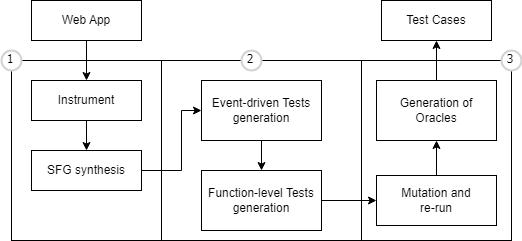
\includegraphics[width=.99\textwidth]{Figures/jseft2.png}
  \caption{JSEFT structure}\label{fig:jseft}
\end{figure}

For the export of event-driven and function-level tests, the frameworks Selenium\footnote{https://www.selenium.dev} and QUnit\footnote{https://qunitjs.com} are used respectively.

The experiment section of the author's paper, shows the study of JSEFT's usage on 13 JavaScript web applications so the line coverage and usefulness of the assertions at the time of finding regression faults.
For the specified metrics, the tool got a \(68.4\%\) of line coverage and a \(100\%\) precision in fault detection.

\chapter{Conclusions}~\label{chap:conclusions}

Through the conducted study, a Python implementation for Pynguin of the Graph Based Object Synthesis heuristic was presented for the generation of the previously defined complex object inputs.
The expectation from the experiments aimed for an improvement in branch coverage results when running the approach into a set of Python modules, that served as generalization of the common publicly available Python module.
Although, this prediction had the heuristic's original result on its Java implementation of a Cohen's D effect size improvement of \(0.21\) as baseline, the observed effect size in the general results presented a different outcome, with a negative value of \(\AverageCohen\).

At the same time, the introduced metric ``OLR'' helped as an intermediary measure for the presence of a need for complex object inputs within Python modules. 
Nonetheless, not even by focusing the efforts of the experimental setup on those Python modules that had a greater OLR, any improvement was found at all, getting an average \(\hat{A}_{12}\) Vargha-Delaney effect size of \(\AverageA\).
This behaviour was analysed further with the idea of a possible correlation between the OLR and the improvement when using the GBOS approach, which was completely refuted by the computation of both Pearson's and Spearman's correlation coefficients.

While the presented approach did not improve Pynguin's results on the set of Python modules beforehand, this might as well describe the current state of the usage of Python as a programming language, implying that even though there are many resources for a correct typing within the dynamically typed language, most developers still do not make full usage of them.
The latter statement is made based on the results of the OLR histogram, exhibited in Figure~\ref{fig:olr-hist}, explaining a general lack of explicit type information regarding callable parameters.

With this last point, it would be reasonable to propose a repetition of the current study and its experimental setup sometime in the future, whenever there might be a change in Python's developer community over the way explicit type information is handled.
Besides, there were many specific scenarios regarding the type annotation gathering system or from the PDG generation that were not taken into account, and will be mentioned in the following section.

\section{Future Work}

Considering the various challenges encountered during the coding of Pynguin's GBOS extension, there are many possible updates and subsequent approached that could be tried and are left as the proposed future work.

One of them, is the improvement of the \classname{DataDependenceGraph}, specifically during its computation and the execution of stack frame effects coming from the different instruction in the CFG.\@
The idea for this point would be to add into the dictionary of \classname{Frame} instances, a tuple or collection instead of a single frame for those nodes that contain an instruction with different stack frame states depending on the presence of an Exception.

Another idea that might be worth diving into, is the addition of functions into the interprocedural analysis (see Section~\ref{sec:pdgia}) made before the construction of the OCG.\@
Here, a possible update would need to ideate a way to link every argument from the Python Bytecode relevant for a function call, with the corresponding variable names in the function's particular sub PDG.\@

Although it has not been mentioned before so far, considering the GBOS specific times regarding execution, it could be possible that further optimization of the developed code might improve some computation overhead produced by the heuristic e.g.~by saving the interprocedural PDG generated for a branch to be reused in another one that belongs to a same code object.

Finally, one factor that would make the GBOS heuristic much more appliable to a general case, is the ability to not depend on explicit type annotations.
This could be achieved in many ways, but considering the ongoing discovery of diverse application for LLMs and the good results obtained by the state-of-the-art automatic test generation tools that use this technology, it is safe to say applying one of the models might a first approach.

\backmatter{}

\printbibliography{}

\end{document}
